%=============================================================================
%  Universal Analyst - Technical Documentation
%  DEPI Graduation Project - LLM-Driven Data Analysis
%
%  Compile on Overleaf (or locally) with pdfLaTeX.  Recommended:
%      latexmk -pdf main.tex          (runs enough passes for TOC/refs)
%  or three pdfLaTeX passes.
%
%  This is the MASTER file. Chapters live in ./chapters and are pulled in
%  with \input near the bottom. Fonts, colours, and styling are defined here.
%=============================================================================
\documentclass[11pt,a4paper,oneside]{report}

%------------------------------------------------------------------ encoding
\usepackage[T1]{fontenc}
\usepackage[utf8]{inputenc}

%--------------------------------------------------------------------- fonts
% Palatino-flavoured text + math: warm, "document" feel, highly readable.
\usepackage{newpxtext}
\usepackage{newpxmath}
\usepackage[scaled=0.85]{beramono} % clean monospace for code
\linespread{1.06}

%------------------------------------------------------------------- geometry
\usepackage[a4paper,margin=1in,headheight=15pt,footskip=32pt]{geometry}

%-------------------------------------------------------------------- colours
\usepackage{xcolor}
\definecolor{uaIndigo}{RGB}{79,70,229}     % primary action / identity
\definecolor{uaIndigoD}{RGB}{49,46,129}    % deep indigo
\definecolor{uaAmber}{RGB}{217,119,6}      % measurement / emphasis
\definecolor{uaInk}{RGB}{17,24,39}         % near-black body ink
\definecolor{uaSlate}{RGB}{71,85,105}      % secondary text
\definecolor{uaMist}{RGB}{241,245,249}     % pale panel fill
\definecolor{uaLine}{RGB}{203,213,225}     % hairline rules
\definecolor{uaGreen}{RGB}{16,150,110}     % success / positive
\definecolor{uaCode}{RGB}{30,41,59}        % code text
\definecolor{uaCodeBg}{RGB}{248,250,252}   % code background
\definecolor{uaKw}{RGB}{124,58,237}        % code keyword
\definecolor{uaStr}{RGB}{5,150,105}        % code string
\definecolor{uaCom}{RGB}{100,116,139}      % code comment

%------------------------------------------------------------------- graphics
\usepackage{graphicx}
\usepackage{tikz}
\usetikzlibrary{positioning,arrows.meta,calc,shapes.geometric,backgrounds,fit,shadows.blur}
\usepackage{pgfplots}
\pgfplotsset{compat=1.17}

%---------------------------------------------------------------------- boxes
\usepackage[most]{tcolorbox}

%----------------------------------------------------------------- tables etc
\usepackage{booktabs}
\usepackage{array}
\usepackage{tabularx}
\usepackage{multirow}
\usepackage{longtable}
\usepackage{ragged2e}
\newcolumntype{L}[1]{>{\RaggedRight\arraybackslash}p{#1}}
\newcolumntype{C}[1]{>{\Centering\arraybackslash}p{#1}}

%--------------------------------------------------------------------- misc
\usepackage{enumitem}
\setlist{itemsep=2pt,topsep=4pt,parsep=0pt}
\usepackage{fancyhdr}
\usepackage{titlesec}
\usepackage{listings}
\usepackage{caption}
\captionsetup{font=small,labelfont={bf,color=uaIndigoD},labelsep=period}
\usepackage[hidelinks]{hyperref}
\hypersetup{
  colorlinks=true,
  linkcolor=uaIndigoD,
  urlcolor=uaIndigo,
  citecolor=uaIndigoD,
  pdftitle={Universal Analyst - Technical Documentation},
  pdfauthor={DEPI Graduation Team},
}
\usepackage{bookmark}
\usepackage{microtype}

%============================== section styling ==============================
\titleformat{\chapter}[display]
  {\normalfont\huge\bfseries\color{uaIndigoD}}
  {\raisebox{-2pt}{\tikz\node[fill=uaIndigo,text=white,rounded corners=3pt,
     inner xsep=8pt,inner ysep=4pt,font=\Large\bfseries]{Chapter \thechapter};}}
  {14pt}
  {\Huge}
  [\vspace{4pt}{\color{uaLine}\titlerule[1.2pt]}]

\titlespacing*{\chapter}{0pt}{-18pt}{22pt}

\titleformat{\section}
  {\normalfont\Large\bfseries\color{uaInk}}
  {\color{uaAmber}\thesection}{0.7em}{}
\titleformat{\subsection}
  {\normalfont\large\bfseries\color{uaSlate}}
  {\color{uaAmber}\thesubsection}{0.6em}{}

%================================ headers/footers =============================
\pagestyle{fancy}
\fancyhf{}
\renewcommand{\headrulewidth}{0.4pt}
\renewcommand{\footrulewidth}{0pt}
\fancyhead[L]{\footnotesize\color{uaSlate}\textsc{Universal Analyst}}
\fancyhead[R]{\footnotesize\color{uaSlate}\leftmark}
\fancyfoot[C]{\footnotesize\color{uaSlate}\thepage}
\fancypagestyle{plain}{\fancyhf{}\fancyfoot[C]{\footnotesize\color{uaSlate}\thepage}\renewcommand{\headrulewidth}{0pt}}
\renewcommand{\chaptermark}[1]{\markboth{\thechapter.\ #1}{}}

%================================ code listings ==============================
\lstdefinestyle{ua}{
  backgroundcolor=\color{uaCodeBg},
  basicstyle=\ttfamily\footnotesize\color{uaCode},
  keywordstyle=\color{uaKw}\bfseries,
  stringstyle=\color{uaStr},
  commentstyle=\color{uaCom}\itshape,
  numberstyle=\tiny\color{uaSlate},
  numbers=left,
  numbersep=8pt,
  stepnumber=1,
  frame=leftline,
  framerule=1.4pt,
  rulecolor=\color{uaIndigo},
  framexleftmargin=6pt,
  xleftmargin=14pt,
  breaklines=true,
  breakatwhitespace=true,
  showstringspaces=false,
  tabsize=2,
  columns=fullflexible,
  keepspaces=true,
  aboveskip=10pt,
  belowskip=8pt,
}
\lstset{style=ua}

% Language-flavoured aliases
\lstdefinestyle{py}{style=ua,language=Python,morekeywords={async,await,self,None,True,False}}
\lstdefinestyle{js}{style=ua,morekeywords={const,let,var,await,async,export,import,from,return,switch,case,new}}
\lstdefinestyle{bash}{style=ua,morekeywords={make,npm,pip,git,cd,bash,uvicorn,run,docker,host}}
\lstdefinestyle{jsonc}{style=ua,morekeywords={true,false,null}}

% Inline code helper: \code{...}
\newcommand{\code}[1]{{\ttfamily\small\color{uaCode}#1}}

%============================== callout boxes ================================
\newtcolorbox{uanote}[1][]{
  enhanced,breakable,
  colback=uaMist,colframe=uaIndigo,
  boxrule=0pt,leftrule=3pt,
  arc=2pt,left=10pt,right=10pt,top=7pt,bottom=7pt,
  fonttitle=\bfseries\color{uaIndigoD},
  title={#1}}

\newtcolorbox{uawarn}[1][]{
  enhanced,breakable,
  colback=uaCodeBg,colframe=uaAmber,
  boxrule=0pt,leftrule=3pt,
  arc=2pt,left=10pt,right=10pt,top=7pt,bottom=7pt,
  fonttitle=\bfseries\color{uaAmber},
  title={#1}}

\newtcolorbox{uakey}[1][]{
  enhanced,breakable,
  colback=white,colframe=uaLine,
  boxrule=0.8pt,arc=3pt,
  left=10pt,right=10pt,top=8pt,bottom=8pt,
  fonttitle=\bfseries\color{uaIndigoD},
  title={#1}}

% A compact "feature" chip
\newcommand{\chip}[1]{\tikz[baseline=(x.base)]\node[fill=uaIndigo!12,draw=uaIndigo!40,
  rounded corners=2pt,inner xsep=4pt,inner ysep=1.5pt,font=\footnotesize\ttfamily,
  text=uaIndigoD](x){#1};}

%============================== TikZ block styles ============================
\tikzset{
  ua-fe/.style={draw=uaIndigo,fill=uaIndigo!10,rounded corners=4pt,
    text=uaInk,align=center,font=\small\bfseries,inner sep=7pt,minimum height=13mm},
  ua-be/.style={draw=uaGreen,fill=uaGreen!10,rounded corners=4pt,
    text=uaInk,align=center,font=\small\bfseries,inner sep=7pt,minimum height=13mm},
  ua-ai/.style={draw=uaAmber,fill=uaAmber!12,rounded corners=4pt,
    text=uaInk,align=center,font=\small\bfseries,inner sep=7pt,minimum height=13mm},
  ua-out/.style={draw=uaIndigoD,fill=uaIndigoD!10,rounded corners=4pt,
    text=uaInk,align=center,font=\small\bfseries,inner sep=7pt,minimum height=13mm},
  ua-arrow/.style={-{Stealth[length=3mm]},uaSlate,thick},
  ua-arrowl/.style={-{Stealth[length=3mm]},uaAmber,thick,dashed},
}

%=============================================================================
\begin{document}
\hypersetup{pageanchor=false}
%=============================================================================
%  00_cover.tex  -  Full-bleed cover page
%=============================================================================
\begin{titlepage}
\thispagestyle{empty}

\begin{tikzpicture}[remember picture, overlay]

  % ---- background ----
  \fill[uaInk] (current page.south west) rectangle (current page.north east);

  % ---- soft indigo glow (top-right) ----
  \begin{scope}
    \clip (current page.south west) rectangle (current page.north east);
    \fill[uaIndigo,opacity=0.16] ([xshift=4cm,yshift=3cm]current page.north east) circle (7cm);
    \fill[uaAmber,opacity=0.10] ([xshift=-3cm,yshift=-4cm]current page.south west) circle (6cm);
  \end{scope}

  % ---- top hairline + eyebrow ----
  \draw[uaAmber,line width=1.2pt]
     ([xshift=1in,yshift=-1.25in]current page.north west) --
     ([xshift=-1in,yshift=-1.25in]current page.north east);
  \node[anchor=west,text=uaAmber,font=\sffamily\bfseries\large]
     at ([xshift=1in,yshift=-1.05in]current page.north west)
     {DEPI \; GRADUATION \; PROJECT};
  \node[anchor=east,text=white!70,font=\sffamily\small]
     at ([xshift=-1in,yshift=-1.05in]current page.north east)
     {LLM for Data Analysis};

  % ---- emblem: concentric arcs + data->model->insight nodes ----
  \begin{scope}[shift={([yshift=-3.7in]current page.north)}]
    \foreach \r/\o in {2.15/0.22, 1.7/0.32, 1.25/0.5} {
      \draw[uaIndigo,opacity=\o,line width=1.1pt] (0,0) circle (\r);
    }
    \draw[uaAmber,line width=1.4pt,opacity=0.9] (0,0) circle (0.8);
    \node[circle,fill=uaAmber,inner sep=2.1pt] at (150:0.8) {};
    \node[circle,fill=white,inner sep=1.6pt] at (30:1.25) {};
    \node[circle,fill=uaIndigo,inner sep=2.1pt] at (-90:1.7) {};
    \node[text=white!85,font=\ttfamily\scriptsize] at (0,0) {analyst};
  \end{scope}

  % ---- title block ----
  \node[anchor=north,text=white,font=\sffamily\bfseries\fontsize{52}{56}\selectfont]
     at ([yshift=-5.1in]current page.north) {Universal Analyst};
  \node[anchor=north,text=uaIndigo!85,font=\sffamily\bfseries\Large]
     at ([yshift=-5.95in]current page.north) {An LLM-Driven Data Analysis Workspace};
  \node[anchor=north,text=white!62,font=\itshape\large,align=center,text width=13cm]
     at ([yshift=-6.5in]current page.north)
     {Upload a dataset. Interrogate it in natural language. Get grounded answers,\\
      model-generated dashboards, and a professional PDF report --- powered by a\\
      \emph{local} multimodal large language model.};

  % ---- tech ribbon ----
  \node[anchor=north,font=\ttfamily\small,text=white!80,align=center,text width=15cm]
     at ([yshift=-7.7in]current page.north)
     {\colorbox{uaIndigo!25}{\strut\ FastAPI\ }\;
      \colorbox{uaIndigo!25}{\strut\ React + Vite\ }\;
      \colorbox{uaAmber!30}{\strut\ Ollama - Gemma\,4\ }\;
      \colorbox{uaIndigo!25}{\strut\ ChromaDB\ }\;
      \colorbox{uaAmber!30}{\strut\ Plotly\ }};

  % ---- bottom plate ----
  \fill[white,opacity=0.04]
     ([xshift=1in,yshift=1.05in]current page.south west) rectangle
     ([xshift=-1in,yshift=2.25in]current page.south east);
  \draw[uaIndigo,opacity=0.5,line width=0.8pt]
     ([xshift=1in,yshift=2.25in]current page.south west) --
     ([xshift=-1in,yshift=2.25in]current page.south east);

  \node[anchor=north west,text=white!60,font=\sffamily\footnotesize\bfseries]
     at ([xshift=1.15in,yshift=2.05in]current page.south west) {PROJECT TEAM};
  \node[anchor=north west,text=white!85,font=\small,align=left]
     at ([xshift=1.15in,yshift=1.78in]current page.south west)
     {Ahmed \;\textbf{\textcolor{white!55}{--}}\; Frontend \\
      Amir \;\textbf{\textcolor{white!55}{--}}\; Backend Core \& LLM \\
      Shahenda \;\textbf{\textcolor{white!55}{--}}\; AI \& RAG};
  \node[anchor=north west,text=white!85,font=\small,align=left]
     at ([xshift=4.7in,yshift=1.78in]current page.south west)
     {Doaa \;\textbf{\textcolor{white!55}{--}}\; Data Engineering \\
      Maimamoon \;\textbf{\textcolor{white!55}{--}}\; Visualization \& Reporting \\
      Hesham \;\textbf{\textcolor{white!55}{--}}\; ML \& DevOps};

  \node[anchor=south west,text=white!45,font=\ttfamily\scriptsize]
     at ([xshift=1in,yshift=0.6in]current page.south west)
     {Technical Documentation \textbullet\ Version 1.0};
  \node[anchor=south east,text=white!45,font=\ttfamily\scriptsize]
     at ([xshift=-1in,yshift=0.6in]current page.south east)
     {github.com/Ahmedvip62/Depi-Graduation\_project};

\end{tikzpicture}
\end{titlepage}

\hypersetup{pageanchor=true}

\pagenumbering{roman}
%=============================================================================
%  01_abstract.tex  -  Abstract + document conventions (roman-numbered)
%=============================================================================
\chapter*{Abstract}
\addcontentsline{toc}{chapter}{Abstract}
\markboth{Abstract}{}

\begin{tcolorbox}[enhanced,colback=uaMist,colframe=uaIndigo,boxrule=0pt,leftrule=4pt,
  arc=2pt,left=14pt,right=14pt,top=12pt,bottom=12pt]
\setlength{\parindent}{0pt}
\textbf{\large\color{uaIndigoD}Universal Analyst} is a self-hosted, LLM-driven
workspace that turns any uploaded dataset into an interrogable analytical
instrument. A user uploads a file --- CSV, JSON, Parquet, a PDF containing
tables, or a SQLite database --- and the system automatically \emph{profiles}
the data, runs \emph{exploratory data analysis}, and builds a
\emph{retrieval-augmented} context so that a \emph{local} multimodal large
language model (Gemma\,4, served through Ollama) can answer questions that are
grounded in the actual data rather than in the model's parametric memory.
\end{tcolorbox}

\vspace{6pt}
The platform goes beyond conversational question answering. Through a
router-driven \textbf{skill system}, the same session can request a
model-planned and server-\emph{validated} interactive dashboard, run a
lightweight \textbf{predictive-modeling} pipeline built on scikit-learn, perform
guided data \textbf{cleaning}, or export a branded, professional \textbf{PDF
report} containing the profile, quality signals, generated charts, and the full
conversation transcript. A central design commitment --- the \emph{no-fabrication
rule} --- ensures the interface never substitutes placeholder analysis for real
model output; when the model or the runtime fails, the system reports precisely
what happened.

This document describes the complete system: its motivation and product
philosophy, the end-to-end architecture, and each subsystem in depth ---
ingestion, profiling, chunking, the ChromaDB retrieval layer, the streaming
Ollama client, the six analytical skills, the Plotly chart-validation engine,
the scikit-learn prediction pipeline, the ReportLab PDF generator, the React
front end, the HTTP API surface, containerized deployment, testing, and
security posture. It closes with the team's six-way work split, a roadmap, and
appendices covering configuration and the event protocol.

\vspace{10pt}
\begin{center}

\begin{tikzpicture}
  \node[font=\itshape\large,text=uaSlate] {measured \;\textcolor{uaAmber}{\textbullet}\; grounded \;\textcolor{uaAmber}{\textbullet}\; sharp};
\end{tikzpicture}
\end{center}

\vfill
\subsection*{\color{uaIndigoD}Document Conventions}
\begin{itemize}
  \item \code{Inline monospace} denotes code identifiers, file names, endpoints,
        and configuration keys.
  \item Full code listings are drawn from the project's actual source and are
        line-numbered with an indigo margin rule.
  \item \textbf{Blue callouts} highlight design rationale; \textbf{amber
        callouts} flag constraints, caveats, and operational warnings.
  \item Figures render as vector diagrams; every figure and table is listed in
        the front matter.
\end{itemize}


% ---- front matter listings ----
\clearpage
\pagestyle{plain}
\tableofcontents
\clearpage
\listoffigures
\clearpage
\listoftables
\clearpage
\pagestyle{fancy}
\pagenumbering{arabic}
\setcounter{page}{1}

% ============================ main matter ============================
%=============================================================================
%  02_introduction.tex  -  Chapter 1: Introduction
%=============================================================================
\chapter{Introduction}
\label{ch:intro}

\section{Motivation}
The last few years have made it trivially easy to \emph{ask a language model a
question}, and correspondingly easy for that model to answer with fluent,
confident, and \emph{wrong} numbers. For data analysis this failure mode is
particularly dangerous: a plausible-looking figure or a neat chart carries an
authority that a paragraph of prose does not. A tool that ``chats with your
data'' is only useful if the analyst can trust that what it reports is actually
\emph{in} the data.

Universal Analyst is built around that trust problem. Rather than treating the
language model as an oracle, it treats it as a \emph{reasoning engine wrapped in
guardrails}: the data is profiled deterministically, relevant facts are
retrieved from a vector index built from the user's own file, and every chart
the model proposes is validated against the real schema before it is rendered.
The model plans; the system verifies; the interface never fakes.

\begin{uanote}[The core promise]
Given a dataset and a question, the analyst gets a correct, grounded answer or a
real chart --- \emph{fast} --- and can trust that nothing was fabricated. Empty
states and error states say what actually happened.
\end{uanote}

\section{Problem Statement}
Existing ``AI + data'' tools tend to fall into one of three traps:

\begin{enumerate}
  \item \textbf{Hallucinated analysis.} The model invents statistics or trends
        that are not supported by the data, because it never actually reads the
        data --- only a truncated preview or nothing at all.
  \item \textbf{Cloud dependence.} The dataset is shipped to a third-party API,
        raising privacy, cost, and reproducibility concerns that are
        unacceptable for many analysts and organizations.
  \item \textbf{Decorative dashboards.} Charts are generated from templates that
        look impressive but are disconnected from the underlying columns, or are
        silently substituted when the model fails.
\end{enumerate}

Universal Analyst addresses all three: it grounds answers in retrieval over the
uploaded data, it runs the model entirely \emph{locally} on the user's GPU
runtime, and it renders only charts that survive a strict server-side
validation pass.

\section{Objectives}
\begin{table}[h]
\centering
\caption{Primary project objectives and how they are met.}
\begin{tabularx}{\linewidth}{@{}L{4.7cm} X@{}}
\toprule
\textbf{Objective} & \textbf{Realization in the system} \\
\midrule
Grounded question answering & RAG over a per-session ChromaDB index built from
schema, per-column, and row chunks of the uploaded file. \\
Local, private inference & Gemma\,4 (12B primary, \code{e4b} router) served via
Ollama on the same GPU box; no data leaves the runtime. \\
Trustworthy visualization & The model emits a strict chart \emph{plan}; the
\code{ChartFactory} validates columns and types before rendering Plotly. \\
Multi-format ingestion & A single \code{IngestionEngine} handling CSV, JSON,
Parquet, PDF tables, and SQLite. \\
Actionable outputs & Skills for cleaning, prediction, and a branded PDF report,
in addition to chat and dashboards. \\
Operational honesty & The \emph{no-fabrication rule}: real streamed output or a
real error, never a placeholder. \\
\bottomrule
\end{tabularx}
\end{table}

\section{Scope}
This project delivers a complete, runnable full-stack application: a Python
\code{3.12} FastAPI backend, a React\,18 single-page front end, a retrieval
layer, a local-LLM integration, a validated visualization engine, a prediction
pipeline, a PDF reporting engine, container definitions for development and
production, a one-click cloud-setup notebook, and a continuous-integration
workflow. It targets a single-analyst, single-session analytical workflow on a
cloud GPU runtime (for example, Lightning.ai). Multi-tenant scaling, persistent
user accounts, and a managed database are explicitly out of scope for this
iteration and are discussed as future work in Chapter~\ref{ch:future}.

\section{Contributions}
\begin{itemize}
  \item A \textbf{grounded analytical assistant} that combines deterministic
        profiling with retrieval-augmented generation over the user's data.
  \item A \textbf{validated, model-driven visualization pipeline} that turns a
        constrained LLM chart plan into a real, correct Plotly figure.
  \item A \textbf{skill-routing architecture} that lets one natural-language
        interface dispatch to analysis, visualization, cleaning, prediction, and
        reporting.
  \item A \textbf{fully local, streaming inference path} with token-level usage
        accounting and multimodal (image) support.
  \item A \textbf{reproducible deployment story} spanning a setup notebook,
        Docker Compose (development and production), and CI.
\end{itemize}

\section{Document Roadmap}
Chapter~\ref{ch:product} frames the product philosophy and users.
Chapter~\ref{ch:arch} presents the end-to-end architecture and request
lifecycle. Chapters~\ref{ch:ingestion}--\ref{ch:reporting} descend into each
backend subsystem in the order data flows through it: ingestion and profiling,
the RAG layer, the LLM client, the skill system, visualization, prediction, and
reporting. Chapter~\ref{ch:frontend} covers the React front end;
Chapter~\ref{ch:api} the HTTP surface; Chapter~\ref{ch:deploy} configuration and
deployment; Chapter~\ref{ch:testing} testing and quality;
Chapter~\ref{ch:security} security and limitations. The document closes with the
team split (Chapter~\ref{ch:team}), future work (Chapter~\ref{ch:future}), a
conclusion, and appendices.

%=============================================================================
%  03_product.tex  -  Chapter 2: Product Philosophy and Users
%=============================================================================
\chapter{Product Philosophy and Users}
\label{ch:product}

\section{Who it is for}
Universal Analyst is built for \textbf{data analysts, data-science students, and
technical operators} who arrive with a concrete dataset and a concrete question.
Their context is a focused analysis session rather than a long-lived project:
they upload data, read the profile, ask grounded questions, request a chart or a
prediction, and export a report. They value \emph{speed}, \emph{density}, and
\emph{trustworthy output} over decoration, and they are fluent in tools like
Linear and Stripe --- so standard product affordances should behave exactly as
they expect.

\begin{table}[h]
\centering
\caption{Primary persona and the job the product does for them.}
\begin{tabularx}{\linewidth}{@{}L{3.4cm} X@{}}
\toprule
\textbf{Persona} & \textbf{Job-to-be-done} \\
\midrule
Data analyst & ``I have this file and a question --- give me a correct,
grounded answer and, if it helps, a real chart, without me writing code.'' \\
DS student & ``Let me explore a dataset's structure, try a quick predictive
model, and produce a clean report I can hand in.'' \\
Technical operator & ``Run this locally on our GPU box; nothing about our data
should leave the machine.'' \\
\bottomrule
\end{tabularx}
\end{table}

\section{Brand personality}
The product is deliberately positioned as an \emph{instrument}, not a marketing
app: precise, technical, and quietly confident. Three words anchor the identity
--- \textbf{measured, grounded, sharp}. It should feel like a piece of lab
equipment a professional reaches for, where every readout is exact and earned:
no hype, no hand-holding, no filler copy.

\section{Design principles}
The following principles govern both the interface and the backend behaviour.
They are not aspirational --- each maps to concrete implementation decisions
described later in this document.

\begin{description}[style=nextline,leftmargin=0pt]
  \item[\textcolor{uaIndigoD}{Readouts are exact.}]
    Numbers, counts, and labels render in a monospaced face (IBM Plex Mono) so
    data reads like instrument output rather than prose. See the front-end
    typography in Chapter~\ref{ch:frontend}.
  \item[\textcolor{uaIndigoD}{Earned familiarity.}]
    Tabs, side navigation, the composer, and tables behave exactly as a
    Linear/Stripe-fluent user expects, so the tool disappears into the task.
  \item[\textcolor{uaIndigoD}{No fabrication.}]
    The UI never substitutes static or placeholder analysis for real model
    output. Empty and error states say what actually happened --- this is
    enforced in the streaming chat path (Chapter~\ref{ch:llm}).
  \item[\textcolor{uaIndigoD}{One signal, one job.}]
    Indigo carries actions, focus, and identity; amber marks measurement and
    emphasis only. Neither colour is used to decorate.
  \item[\textcolor{uaIndigoD}{Density with rhythm.}]
    The interface is information-dense where the analyst needs it, using
    deliberate spacing and hairline structure rather than nested cards.
\end{description}

\begin{uanote}[The no-fabrication rule, concretely]
When the model or Ollama fails mid-answer, the backend emits a real
\code{error} event and the front end shows it verbatim. The system never
back-fills a canned profile summary, a fake chart, or invented statistics to
paper over a failure. This single rule shapes error handling across every
subsystem.
\end{uanote}

\section{Anti-references}
Part of defining a product is defining what it must \emph{not} become. Universal
Analyst explicitly rejects:

\begin{itemize}
  \item The generic AI-SaaS dashboard --- rounded cards everywhere, purple-to-blue
        gradient accents, a tiny uppercase eyebrow over every section, and
        hero-metric templates.
  \item The ``warm cream and terracotta serif'' editorial template (the
        project's original look, explicitly retired).
  \item The flat ``near-black plus one acid-green accent'' dark default; the
        current theme stays differentiated by its indigo/amber duotone and
        monospaced data signature.
  \item Any surface that advertises a capability it does not actually have.
\end{itemize}

\section{Accessibility and inclusion}
The application ships a dark theme in which body text and labels meet WCAG AA
contrast (at least \code{4.5:1}, or \code{3:1} for large text). Every
interactive element has a visible keyboard focus state, all motion has a
\code{prefers-reduced-motion} fallback, and microphone dictation is an optional
enhancement --- never the only path to input. Accessibility is treated as a
correctness property of the interface, not a later polish step.

%=============================================================================
%  04_architecture.tex  -  Chapter 3: System Architecture
%=============================================================================
\chapter{System Architecture}
\label{ch:arch}

\section{Overview}
Universal Analyst is a two-tier application: a React single-page front end and a
FastAPI backend, with the backend orchestrating a set of AI and data
subsystems and delegating language generation to a local Ollama runtime. The
front end never talks to Ollama directly; every capability is mediated by the
backend so that validation, grounding, and the no-fabrication rule can be
enforced in one place.

\begin{figure}[h]
\centering
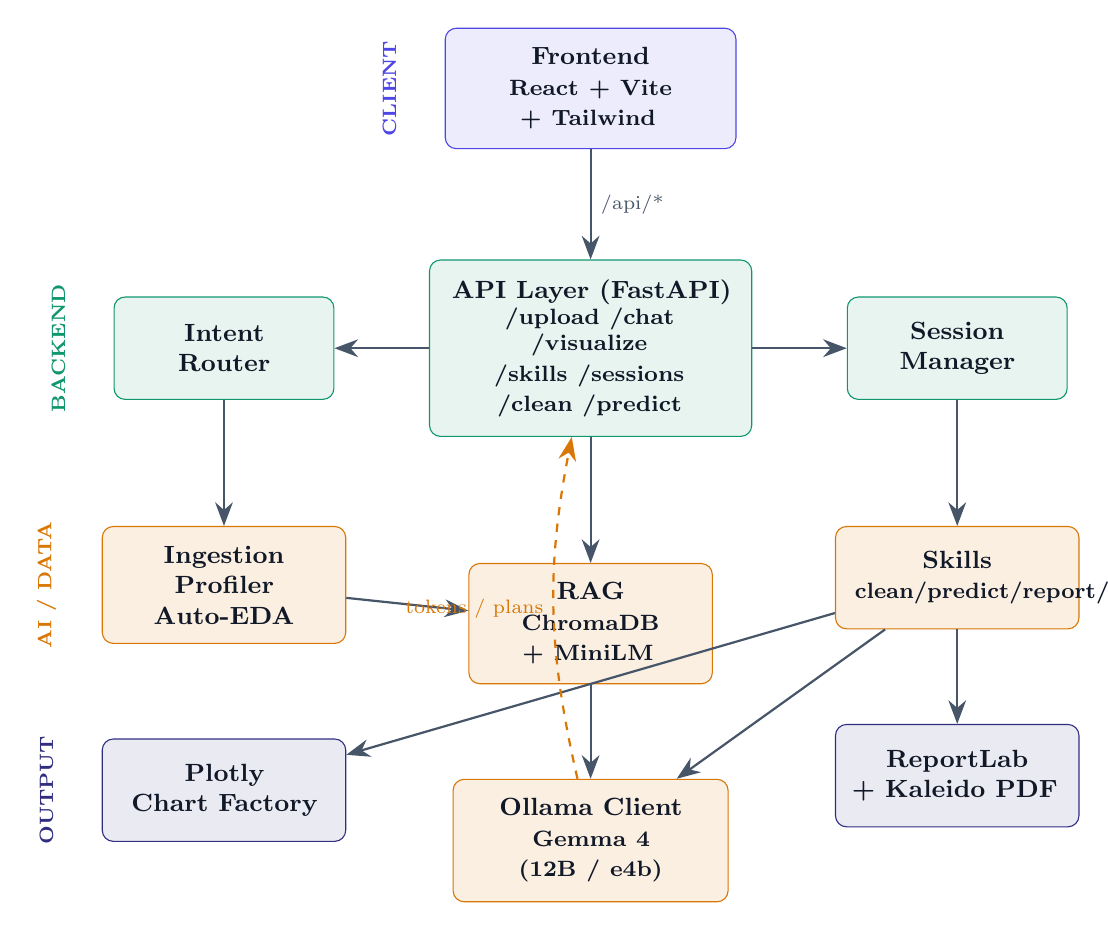
\begin{tikzpicture}[node distance=8mm and 12mm]
  % Frontend
  \node[ua-fe,text width=3.2cm] (ui) {Frontend\\\footnotesize React + Vite + Tailwind};

  % Backend layer
  \node[ua-be,below=14mm of ui,text width=3.6cm] (routes) {API Layer (FastAPI)\\\footnotesize /upload /chat /visualize\\/skills /sessions /clean /predict};
  \node[ua-be,left=of routes,text width=2.3cm] (router) {Intent\\Router};
  \node[ua-be,right=of routes,text width=2.3cm] (sess) {Session\\Manager};

  % AI/data layer
  \node[ua-ai,below=16mm of router,text width=2.6cm] (data) {Ingestion\\Profiler\\Auto-EDA};
  \node[ua-ai,below=16mm of routes,text width=2.6cm] (rag) {RAG\\\footnotesize ChromaDB + MiniLM};
  \node[ua-ai,below=16mm of sess,text width=2.6cm] (skills) {Skills\\\footnotesize clean/predict/report/viz};

  \node[ua-ai,below=12mm of rag,text width=3.0cm] (llm) {Ollama Client\\\footnotesize Gemma 4 (12B / e4b)};

  % Output layer
  \node[ua-out,below=12mm of data,text width=2.6cm] (viz) {Plotly\\Chart Factory};
  \node[ua-out,below=12mm of skills,text width=2.6cm] (pdf) {ReportLab\\+ Kaleido PDF};

  % edges
  \draw[ua-arrow] (ui) -- node[right,font=\scriptsize,text=uaSlate]{/api/*} (routes);
  \draw[ua-arrow] (routes) -- (router);
  \draw[ua-arrow] (routes) -- (sess);
  \draw[ua-arrow] (router) -- (data);
  \draw[ua-arrow] (routes) -- (rag);
  \draw[ua-arrow] (sess) -- (skills);
  \draw[ua-arrow] (data) -- (rag);
  \draw[ua-arrow] (rag) -- (llm);
  \draw[ua-arrow] (skills) -- (llm);
  \draw[ua-arrow] (skills) -- (viz);
  \draw[ua-arrow] (skills) -- (pdf);
  \draw[ua-arrowl] (llm) to[bend left=12] node[left,font=\scriptsize,text=uaAmber]{tokens / plans} (routes);

  % layer labels (anchored to the left-column nodes)
  \node[font=\scriptsize\bfseries,text=uaIndigo,rotate=90] at ([xshift=-7mm]ui.west) {CLIENT};
  \node[font=\scriptsize\bfseries,text=uaGreen,rotate=90] at ([xshift=-7mm]router.west) {BACKEND};
  \node[font=\scriptsize\bfseries,text=uaAmber,rotate=90] at ([xshift=-7mm]data.west) {AI / DATA};
  \node[font=\scriptsize\bfseries,text=uaIndigoD,rotate=90] at ([xshift=-7mm]viz.west) {OUTPUT};
\end{tikzpicture}
\caption{High-level component architecture. The backend is the single point at
which grounding, validation, and the no-fabrication rule are enforced.}
\label{fig:arch}
\end{figure}

\section{Component responsibilities}
\begin{table}[h]
\centering
\caption{Backend packages and their responsibilities.}
\small
\begin{tabularx}{\linewidth}{@{}L{3.2cm} X@{}}
\toprule
\textbf{Package} & \textbf{Responsibility} \\
\midrule
\code{app.api} & HTTP route handlers: chat, upload, sessions, visualizations,
skills, clean, predict, health. \\
\code{app.core} & Ingestion, chunking, profiling, and the in-memory session
manager. \\
\code{app.eda} & Automated exploratory data analysis over the profile. \\
\code{app.llm} & Ollama HTTP client, prompt templates, and token counting. \\
\code{app.rag} & ChromaDB store, sentence-transformers embedder, retriever, and
context builder. \\
\code{app.skills} & Cleaning, prediction, report, and report-narrative
implementations. \\
\code{app.skills\_registry} & Markdown definitions that steer the model per
skill. \\
\code{app.visualization} & Plotly chart factory, chart-type logic, and image
export. \\
\code{app.models} & Pydantic schemas and enumerations shared across the app. \\
\bottomrule
\end{tabularx}
\end{table}

\section{Request lifecycle}
Figure~\ref{fig:lifecycle} traces a full session: an upload that profiles and
indexes the data, a question that is grounded via retrieval and streamed from
the model, an optional chart that is validated before rendering, and a report
export.

\begin{figure}[h]
\centering
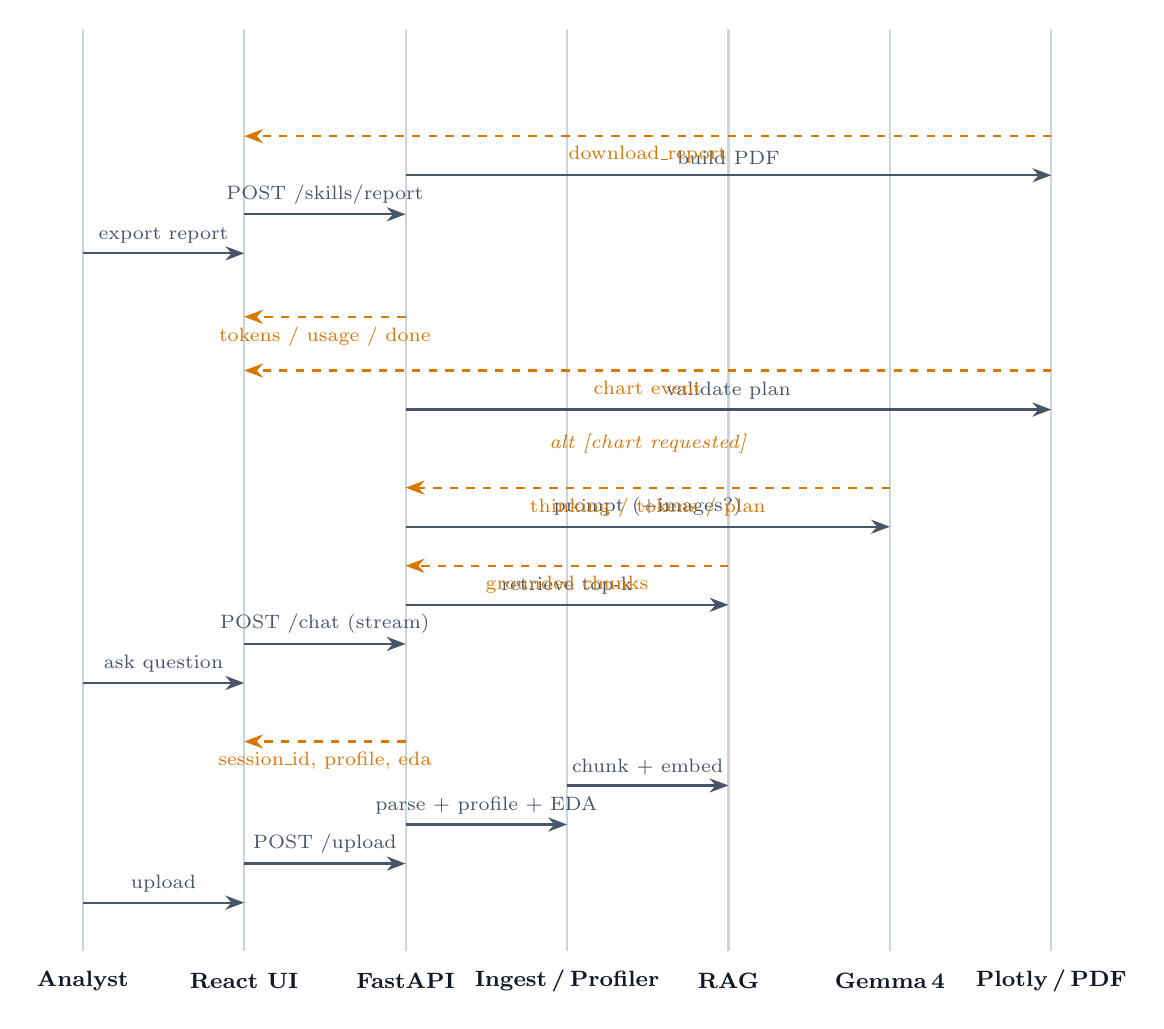
\begin{tikzpicture}[
  actor/.style={font=\footnotesize\bfseries,text=uaInk},
  lifeline/.style={uaLine,thick},
  msg/.style={-{Stealth[length=2.4mm]},uaSlate,thick,font=\scriptsize},
  ret/.style={-{Stealth[length=2.4mm]},uaAmber,thick,dashed,font=\scriptsize},
  x=2.05cm,y=-0.62cm]

  \foreach \i/\name in {0/Analyst,1/{React UI},2/FastAPI,3/{Ingest\,/\,Profiler},4/{RAG},5/{Gemma\,4},6/{Plotly\,/\,PDF}}{
    \node[actor] (h\i) at (\i,0) {\name};
    \draw[lifeline] (\i,-0.6) -- (\i,-19.5);
  }

  \draw[msg] (0,-1.6) -- node[above]{upload} (1,-1.6);
  \draw[msg] (1,-2.4) -- node[above]{POST /upload} (2,-2.4);
  \draw[msg] (2,-3.2) -- node[above]{parse + profile + EDA} (3,-3.2);
  \draw[msg] (3,-4.0) -- node[above]{chunk + embed} (4,-4.0);
  \draw[ret] (2,-4.9) -- node[below]{session\_id, profile, eda} (1,-4.9);

  \draw[msg] (0,-6.1) -- node[above]{ask question} (1,-6.1);
  \draw[msg] (1,-6.9) -- node[above]{POST /chat (stream)} (2,-6.9);
  \draw[msg] (2,-7.7) -- node[above]{retrieve top-k} (4,-7.7);
  \draw[ret] (4,-8.5) -- node[below]{grounded chunks} (2,-8.5);
  \draw[msg] (2,-9.3) -- node[above]{prompt (+images?)} (5,-9.3);
  \draw[ret] (5,-10.1) -- node[below]{thinking / tokens / plan} (2,-10.1);

  \node[font=\scriptsize\itshape,text=uaAmber] at (3.5,-11.0) {alt [chart requested]};
  \draw[msg] (2,-11.7) -- node[above]{validate plan} (6,-11.7);
  \draw[ret] (6,-12.5) -- node[below]{chart event} (1,-12.5);

  \draw[ret] (2,-13.6) -- node[below]{tokens / usage / done} (1,-13.6);

  \draw[msg] (0,-14.9) -- node[above]{export report} (1,-14.9);
  \draw[msg] (1,-15.7) -- node[above]{POST /skills/report} (2,-15.7);
  \draw[msg] (2,-16.5) -- node[above]{build PDF} (6,-16.5);
  \draw[ret] (6,-17.3) -- node[below]{download\_report} (1,-17.3);
\end{tikzpicture}
\caption{End-to-end request lifecycle, from upload to grounded answer to report
export. Dashed amber arrows are streamed or returned responses.}
\label{fig:lifecycle}
\end{figure}

\section{Routing and paths}
The backend serves its routes at the root of port \code{8000}. The front end,
however, always calls paths under \code{/api/*}. In every deployment mode a
proxy --- the Vite dev server in development, nginx in production, and a small
forwarding server in the notebook --- rewrites \code{/api/*} onto the backend
while stripping the \code{/api} prefix. This keeps the front-end code identical
across environments and avoids hard-coding backend hostnames.

\begin{uanote}[Why a single mediating backend]
Because grounding (retrieval), validation (chart plans), token accounting, and
error honesty all live behind one API, the front end can stay thin and the
guarantees stay consistent. There is exactly one place where a chart can be
rejected or an error surfaced --- not several.
\end{uanote}

\section{Deployment topology}
Three runtime shapes are supported from the same codebase, summarized in
Table~\ref{tab:topology} and detailed in Chapter~\ref{ch:deploy}.

\begin{table}[h]
\centering
\caption{Supported deployment topologies.}
\label{tab:topology}
\small
\begin{tabularx}{\linewidth}{@{}L{2.7cm} L{3.2cm} X@{}}
\toprule
\textbf{Mode} & \textbf{Front end} & \textbf{Notes} \\
\midrule
Notebook (cloud) & Forwarded Vite dev server & \code{main.ipynb} installs deps,
pulls the Gemma tags, and starts both services on a GPU box. \\
Docker (dev) & Vite dev server in a Node image & Bind-mounts source; Ollama runs
on the host via \code{host.docker.internal}. \\
Docker (prod) & Built static assets behind nginx & \code{docker-compose.prod.yml}
serves optimized images. \\
\bottomrule
\end{tabularx}
\end{table}

%=============================================================================
%  05_ingestion.tex  -  Chapter 4: Data Ingestion and Profiling
%=============================================================================
\chapter{Data Ingestion and Profiling}
\label{ch:ingestion}

The journey of every dataset begins here. Before the language model sees
anything, the backend must turn an arbitrary uploaded file into a clean
\code{pandas.DataFrame}, understand its structure, and describe it in a form that
is both machine-usable (for retrieval) and human-readable (for the profile
panel and the report).

\section{The ingestion engine}
The \code{IngestionEngine} accepts raw bytes plus a filename and dispatches on
the file extension. Five formats are supported, declared explicitly so that an
unsupported upload fails with a clear message rather than a stack trace.

\begin{table}[h]
\centering
\caption{Supported input formats and their parsing strategy.}
\begin{tabularx}{\linewidth}{@{}L{2.4cm} L{2.2cm} X@{}}
\toprule
\textbf{Format} & \textbf{Extension} & \textbf{Strategy} \\
\midrule
CSV & \code{.csv} & \code{pandas.read\_csv} over an in-memory buffer. \\
JSON & \code{.json} & Tolerant parse: arrays become rows, single objects are
normalized, NDJSON is a fallback. \\
Parquet & \code{.parquet} & \code{pandas.read\_parquet} (pyarrow). \\
PDF & \code{.pdf} & \code{pdfplumber} extracts tables page-by-page. \\
SQLite & \code{.sqlite}, \code{.db} & \code{sqlite3} reads all tables; the
largest is used. \\
\bottomrule
\end{tabularx}
\end{table}

\begin{lstlisting}[style=py,caption={Format dispatch in \code{IngestionEngine.parse\_file}.}]
SUPPORTED_EXTENSIONS = {"csv", "json", "parquet", "pdf", "sqlite", "db"}

class IngestionEngine:
    @staticmethod
    def parse_file(file_bytes: bytes, filename: str) -> pd.DataFrame:
        extension = filename.rsplit(".", 1)[-1].lower() if "." in filename else ""

        if extension == "csv":
            try:
                return pd.read_csv(io.BytesIO(file_bytes))
            except Exception as exc:
                raise ValueError(f"Could not read CSV file: {exc}") from exc
        elif extension == "json":
            return IngestionEngine._parse_json(file_bytes)
        elif extension == "parquet":
            return pd.read_parquet(io.BytesIO(file_bytes))
        elif extension == "pdf":
            return IngestionEngine._parse_pdf(file_bytes)
        elif extension in ("sqlite", "db"):
            return IngestionEngine._parse_sqlite(file_bytes)
        else:
            raise ValueError(
                f"Unsupported file format: '{extension}'. "
                f"Supported: {SUPPORTED_EXTENSIONS}")
\end{lstlisting}

\subsection{Tolerant JSON parsing}
JSON is the least predictable of the tabular formats. The engine accepts three
shapes: a top-level array of records (each object becomes a row via
\code{json\_normalize}), a single object (normalized to one row, or expanded when
its values are equal-length lists), and newline-delimited JSON (detected as a
fallback when a strict parse fails). A \code{utf-8-sig} decode transparently
strips a byte-order mark if present.

\subsection{PDF table extraction}
For PDF uploads the engine walks every page with \code{pdfplumber} and calls
\code{extract\_tables}. Header-only or empty tables are skipped; rows whose
column count does not match the header are filtered out. When multiple tables
share an identical column set they are concatenated; otherwise the largest table
is returned. This heuristic favours the single most substantial table in a
document rather than fragile multi-table stitching.

\subsection{SQLite handling}
Because \code{sqlite3} requires a file on disk, the engine writes the uploaded
bytes to a temporary file, enumerates user tables from \code{sqlite\_master},
reads each into a DataFrame, and returns the one with the most rows. The
temporary file is always removed in a \code{finally} block, and a corrupt or
non-database file yields a clear \code{ValueError} rather than a raw driver
error.

\begin{uawarn}[One table per upload]
Both the PDF and SQLite paths deliberately reduce a multi-table source to a
single DataFrame (the largest). This keeps the downstream profile, retrieval
index, and charts unambiguous. Analysing several tables from one file is noted
as future work.
\end{uawarn}

\section{The data profiler}
Once a DataFrame exists, the \code{DataProfiler} produces a
\code{DataProfile} --- a structured, JSON-safe description consumed by the
front-end overview panel, the RAG context, the chart planner, and the PDF
report. Profiling is entirely deterministic: no model is involved.

\subsection{Semantic typing}
Beyond the raw pandas dtype, the profiler assigns each column a \emph{semantic
type}, which is what actually drives chart selection and analysis. The
classification cascade is:

\begin{enumerate}
  \item \textbf{boolean} --- a true boolean dtype, or a two-value string column
        whose tokens are all boolean-like (\code{true/false}, \code{yes/no},
        \code{y/n}, \code{0/1}, \code{on/off}).
  \item \textbf{datetime} --- a native datetime dtype, or an object column that
        parses to a date for more than 80\% of a 200-row sample.
  \item \textbf{id} --- uniqueness above 0.9 combined with either an
        ``id''-bearing name or an integer-like dtype.
  \item \textbf{continuous} --- any other numeric column.
  \item \textbf{categorical} / \textbf{text} --- object columns split by
        cardinality against a \code{max(20, 5\% of rows)} threshold.
\end{enumerate}

\begin{lstlisting}[style=py,caption={Excerpt of the semantic-type cascade in \code{DataProfiler}.}]
if pd.api.types.is_bool_dtype(series):
    return "boolean"
if not pd.api.types.is_numeric_dtype(series) and DataProfiler._looks_boolean(series):
    return "boolean"
if pd.api.types.is_datetime64_any_dtype(series):
    return "datetime"
# ... object-that-parses -> datetime ...
uniqueness = (unique_count / row_count) if row_count else 0.0
name_has_id = "id" in str(name).lower()
integer_like = pd.api.types.is_integer_dtype(series)
if uniqueness > 0.9 and (name_has_id or integer_like):
    return "id"
if is_numeric:
    return "continuous"
\end{lstlisting}

\subsection{Per-column statistics}
For continuous and id columns the profiler records min, max, mean, median,
standard deviation, \textbf{skewness}, and an \textbf{IQR-based outlier count}
(values beyond $Q_1 - 1.5\,\mathrm{IQR}$ or $Q_3 + 1.5\,\mathrm{IQR}$). Datetime
columns contribute ISO-formatted min/max. Categorical, id, and boolean columns
record their top five values with counts. Every value passes through a
\code{\_json\_safe} helper that converts numpy and pandas scalars, timestamps,
and NaNs into plain JSON primitives --- essential because this profile is
serialized to the front end and embedded in prompts.

\begin{table}[h]
\centering
\caption{Fields captured per column in \code{ColumnProfile}.}
\small
\begin{tabularx}{\linewidth}{@{}L{4.2cm} X@{}}
\toprule
\textbf{Field} & \textbf{Meaning} \\
\midrule
\code{dtype}, \code{semantic\_type} & Raw pandas dtype and inferred role. \\
\code{null\_count}, \code{missing\_pct} & Absolute and percentage missingness. \\
\code{unique\_count} & Distinct non-null values. \\
\code{min/max/mean/median/std} & Summary statistics for numeric columns. \\
\code{skewness}, \code{outlier\_count} & Distribution shape and IQR outliers. \\
\code{sample\_values}, \code{top\_values} & Examples and most-frequent values. \\
\bottomrule
\end{tabularx}
\end{table}

\subsection{Dataset-level signals}
At the whole-table level the profiler computes overall missingness, an estimated
in-memory footprint (\code{memory\_usage(deep=True)}), and --- when at least two
continuous columns exist --- a rounded \textbf{correlation matrix}. It also
publishes convenience lists of the datetime, numeric, and categorical column
names, which the chart planner uses to decide which visualizations are even
possible.

\section{Automated EDA}
Layered on top of the profile, \code{generate\_auto\_eda} assembles a compact
exploratory summary --- human-readable size figures, de-duplicated column
groupings, and headline observations --- that seeds both the overview panel and
the opening context the model receives. Because it is derived from the
deterministic profile, the EDA carries the same trust guarantee: it reflects the
data, not the model's guesswork.

\begin{uanote}[Why deterministic profiling matters]
Everything the model later says about the data is anchored to this profile. By
computing types, statistics, and correlations \emph{without} the LLM, the system
guarantees a stable, reproducible factual base --- the model interprets, it does
not measure.
\end{uanote}

%=============================================================================
%  06_rag.tex  -  Chapter 5: Retrieval-Augmented Generation
%=============================================================================
\chapter{The Retrieval-Augmented Generation Layer}
\label{ch:rag}

Grounding is what separates Universal Analyst from a chatbot that merely
\emph{sounds} authoritative. When the user asks a question, the answer is
assembled from facts retrieved out of \emph{their} dataset, not recalled from
the model's weights. This chapter describes how a DataFrame becomes an
embeddable, queryable index and how that index is turned into a token-budgeted
prompt.

\section{Pipeline overview}
\begin{figure}[h]
\centering
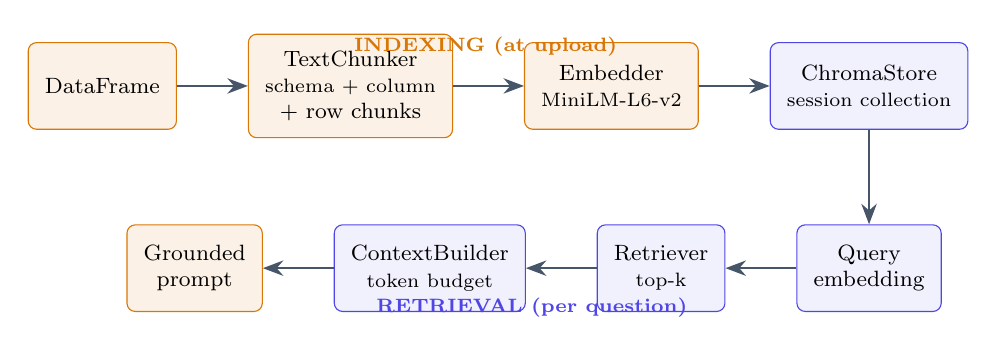
\begin{tikzpicture}[node distance=6mm and 9mm,
  box/.style={draw,rounded corners=3pt,align=center,font=\footnotesize,inner sep=6pt,minimum height=11mm},
  fe/.style={box,draw=uaAmber,fill=uaAmber!10},
  be/.style={box,draw=uaIndigo,fill=uaIndigo!8},
  a/.style={-{Stealth[length=2.6mm]},uaSlate,thick}]
  \node[fe] (df) {DataFrame};
  \node[fe,right=of df] (chunk) {TextChunker\\\scriptsize schema + column\\+ row chunks};
  \node[fe,right=of chunk] (emb) {Embedder\\\scriptsize MiniLM-L6-v2};
  \node[be,right=of emb] (store) {ChromaStore\\\scriptsize session collection};
  \node[be,below=12mm of store] (query) {Query\\embedding};
  \node[be,left=of query] (ret) {Retriever\\\scriptsize top-k};
  \node[be,left=of ret] (ctx) {ContextBuilder\\\scriptsize token budget};
  \node[fe,left=of ctx] (prompt) {Grounded\\prompt};

  \draw[a] (df) -- (chunk);
  \draw[a] (chunk) -- (emb);
  \draw[a] (emb) -- (store);
  \draw[a] (store) -- (query);
  \draw[a] (query) -- (ret);
  \draw[a] (ret) -- (ctx);
  \draw[a] (ctx) -- (prompt);
  \node[font=\scriptsize\bfseries,text=uaAmber] at ([yshift=5mm]$(df)!0.5!(store)$) {INDEXING (at upload)};
  \node[font=\scriptsize\bfseries,text=uaIndigo] at ([yshift=-5mm]$(prompt)!0.5!(query)$) {RETRIEVAL (per question)};
\end{tikzpicture}
\caption{The RAG pipeline. Indexing happens once at upload; retrieval and
context assembly happen on every question.}
\label{fig:rag}
\end{figure}

\section{Chunking strategies}
A DataFrame is not directly embeddable --- it must be turned into text. The
\code{TextChunker} offers several strategies and a \code{combined} mode that is
the workhorse for grounding:

\begin{description}[style=nextline,leftmargin=0pt]
  \item[\textcolor{uaIndigoD}{Schema chunk}] A single chunk describing the whole
    table: row and column counts, and for each column its dtype and number of
    unique values.
  \item[\textcolor{uaIndigoD}{Per-column summary chunks}] One chunk per column
    with descriptive statistics for numeric columns, or the top five values for
    categorical ones, plus null counts.
  \item[\textcolor{uaIndigoD}{Row chunks}] CSV blocks of up to ten rows each,
    capturing the actual records.
\end{description}

\subsection{Bounded, representative row sampling}
A naive row-chunking of a large file would produce tens of thousands of chunks,
all embedded synchronously during the upload request --- a reliable way to hang
or exhaust memory. The chunker therefore enforces a hard cap
(\code{MAX\_ROW\_CHUNKS = 200}). When the dataset would exceed it, the chunker
takes an \emph{evenly-spaced} sample across the whole table rather than only its
head, so the embedded rows still represent the dataset end-to-end.

\begin{lstlisting}[style=py,caption={Bounded, evenly-spaced row sampling.}]
total_chunks = (len(df) + max_rows - 1) // max_rows
if total_chunks <= max_chunks:
    source = df
else:
    # Evenly-spaced rows covering the whole dataset, not just its head.
    step = max(max_rows * (total_chunks // max_chunks), max_rows)
    source = df.iloc[::step].head(max_chunks * max_rows)
\end{lstlisting}

\begin{uanote}[Schema and column chunks are always complete]
Only \emph{row} chunks are sampled. The schema chunk and every per-column
summary are always produced in full, because those are the chunks most useful
for grounding factual answers about structure and distributions.
\end{uanote}

\section{Embeddings}
Chunks are embedded with a \code{sentence-transformers} model,
\code{all-MiniLM-L6-v2} by default, which maps each chunk to a 384-dimensional
vector. The model is loaded \emph{lazily} on first use --- a module-level
singleton --- so that importing the RAG package never triggers a multi-hundred
megabyte download or occupies GPU memory before any data is uploaded.

\begin{lstlisting}[style=py,caption={Lazy singleton loading of the embedding model.}]
_model = None
def _get_model():
    global _model
    if _model is None:
        from sentence_transformers import SentenceTransformer
        from app.config import settings
        _model = SentenceTransformer(settings.embedding_model)
    return _model
\end{lstlisting}

\section{The vector store}
Vectors are persisted in \textbf{ChromaDB} using a \code{PersistentClient}. Each
analysis session gets its own collection, named \code{session\_\{id\}}, so that
retrieval is naturally isolated per dataset and a session can be deleted
cleanly. Like the embedder, the Chroma client is created lazily on first use and
reused thereafter.

\begin{lstlisting}[style=py,caption={Per-session collections in \code{ChromaStore}.}]
class ChromaStore:
    def get_or_create_collection(self, session_id: str):
        client = _get_chroma_client()
        return client.get_or_create_collection(name=f"session_{session_id}")

    def add_chunks(self, session_id, chunks, embeddings):
        collection = self.get_or_create_collection(session_id)
        ids = [f"chunk_{i}" for i in range(len(chunks))]
        collection.add(documents=chunks, embeddings=embeddings, ids=ids)
\end{lstlisting}

When a session is deleted, the session manager also removes the corresponding
Chroma collection --- and does so \emph{outside} its internal lock, because
network or disk I/O should never block other sessions.

\section{Retrieval}
On each question the \code{Retriever} embeds the query and asks the session
collection for the top-$k$ (default five) most similar chunks. It guards
carefully against the empty case: if the collection has no documents --- for
example, a session created before any upload --- it returns an empty list rather
than erroring, and the number of results requested is clamped to the collection
size.

\begin{lstlisting}[style=py,caption={Guarded top-k retrieval.}]
collection = store.get_or_create_collection(session_id)
if collection.count() == 0:
    return []
query_embedding = emb.embed_texts([query])[0]
results = collection.query(
    query_embeddings=[query_embedding],
    n_results=min(top_k, collection.count()))
\end{lstlisting}

\section{Context assembly and the token budget}
Retrieved chunks are not blindly concatenated. The \code{ContextBuilder} owns a
token budget (\code{MAX\_CONTEXT\_TOKENS}, 6000 by default) and spends it
deliberately: it first reserves room for the profile summary, the user's query,
and a fixed margin for the system prompt and the response, then admits retrieved
chunks one at a time until the remaining budget is exhausted.

\begin{lstlisting}[style=py,caption={Token-budgeted context assembly.}]
profile_text = build_profile_summary(profile)
budget = MAX_CONTEXT_TOKENS - count_tokens(profile_text) - count_tokens(query) - 200
trimmed_chunks, used = [], 0
for chunk in chunks:
    t = count_tokens(chunk)
    if used + t > budget:
        break
    trimmed_chunks.append(chunk); used += t
context_str = "\n---\n".join(trimmed_chunks)
return build_data_qa_prompt(query, context_str, profile)
\end{lstlisting}

The result is a single prompt that always contains the deterministic profile
summary and as many relevant, retrieved chunks as the budget allows --- the
raw material from which a grounded answer can be generated.

\begin{uanote}[Grounding is structural, not stylistic]
The model is not merely \emph{asked} to be faithful; it is \emph{given} the
facts. The profile summary and retrieved chunks are the only data-bearing parts
of the prompt, so a faithful answer is the path of least resistance and an
invented one stands out.
\end{uanote}

%=============================================================================
%  07_llm.tex  -  Chapter 6: Local LLM Integration
%=============================================================================
\chapter{Local LLM Integration}
\label{ch:llm}

All language generation happens \emph{locally}, through an Ollama runtime that
serves the Gemma\,4 family. The backend never depends on a remote API; the model
runs on the same GPU box as the application. This chapter covers the two-model
strategy, the streaming client, the event protocol, structured output, and
multimodal input.

\section{A two-model strategy}
Universal Analyst uses two model sizes for two different jobs
(Table~\ref{tab:models}). A large multimodal model answers questions and plans
charts; a small, fast model performs intent routing and classification, where
latency matters more than depth.

\begin{table}[h]
\centering
\caption{The two configured models.}
\label{tab:models}
\small
\begin{tabularx}{\linewidth}{@{}L{3.4cm} L{2.6cm} X@{}}
\toprule
\textbf{Role} & \textbf{Default tag} & \textbf{Used for} \\
\midrule
Primary answering & \code{gemma4:12b} & Grounded answers, chart plans, report
narrative, prediction reasoning; text and images. \\
Router / classifier & \code{gemma4:e4b} & Fast intent routing and lightweight
classification. \\
Embeddings & \code{all-MiniLM-L6-v2} & RAG vectorization (Chapter~\ref{ch:rag}). \\
\bottomrule
\end{tabularx}
\end{table}

\section{The streaming client}
The \code{OllamaClient} wraps Ollama's \code{/api/generate} endpoint using
\code{httpx} with an asynchronous streaming request. Its central method,
\code{generate\_stream\_events}, yields a sequence of typed event dictionaries as
the model produces them. A generous timeout (600\,s total, 10\,s connect)
accommodates cold model loads on a fresh GPU box.

\begin{lstlisting}[style=py,caption={Streaming request construction and per-line event emission.}]
payload = {"model": self.model, "prompt": prompt, "stream": True}
if images:
    payload["images"] = images
if format is not None:
    payload["format"] = format         # "json" or a JSON-schema dict
# ... options: num_predict, temperature ...

async with httpx.AsyncClient(timeout=OLLAMA_TIMEOUT) as client:
    async with client.stream("POST", f"{self.base_url}/generate", json=payload) as response:
        if response.is_error:
            detail = (await response.aread()).decode("utf-8", "replace")[:500]
            yield {"type": "error", "message": f"Ollama request failed ({response.status_code}): {detail}"}
            return
        async for chunk in response.aiter_lines():
            data = json.loads(chunk)
            token = data.get("response")
            if token:
                yield {"type": "token", "token": token}
            if data.get("done"):
                usage = self._usage_from_chunk(data)
                if usage:
                    yield {"type": "usage", "usage": usage}
\end{lstlisting}

\subsection{Honest error propagation}
The client distinguishes three failure modes and, crucially, \emph{never
swallows} them: an HTTP error status yields an \code{error} event with the
status and body excerpt; a mid-stream \code{error} field from Ollama yields an
\code{error} event and stops; and connection or timeout exceptions yield their
own explicit messages. This is the enforcement point for the no-fabrication rule
at the model boundary --- an error becomes a visible error, not a fabricated
answer.

\begin{lstlisting}[style=py,caption={Connection and timeout errors surface as real events.}]
except httpx.ConnectError:
    yield {"type": "error", "message": f"Cannot connect to Ollama at {self.base_url}."}
except httpx.TimeoutException:
    yield {"type": "error", "message": "Ollama request timed out."}
\end{lstlisting}

\subsection{Two consumption modes}
On top of the event generator the client offers two convenience wrappers.
\code{generate\_stream} yields plain token strings for conversational callers;
\code{generate\_text} collects a complete, non-streaming completion and
\emph{raises} on model error. The latter is used by callers that need the whole
response at once and want failures as exceptions --- the chart planner, the
prediction reasoner, and the report narrative generator.

\section{Token accounting}
Ollama reports \code{prompt\_eval\_count} and \code{eval\_count} in its final
chunk. The client's \code{\_usage\_from\_chunk} helper normalizes these into a
\code{usage} record with prompt, completion, and total token counts, and carries
through timing fields (\code{total\_duration}, \code{eval\_duration}, and
related) when present. This usage flows to the front end as a \code{usage} event
so the token meter can display both per-turn and session-level consumption ---
directly serving the ``readouts are exact'' principle.

\section{The chat event protocol}
The \code{/chat} endpoint streams Server-Sent Events, each a small typed JSON
payload. The front end consumes these to render reasoning, tokens, charts, and
usage as they arrive. Table~\ref{tab:events} enumerates the event types.

\begin{table}[h]
\centering
\caption{Streamed chat event types.}
\label{tab:events}
\small
\begin{tabularx}{\linewidth}{@{}L{2.3cm} X@{}}
\toprule
\textbf{Event} & \textbf{Meaning} \\
\midrule
\code{skill} & Which skill the router selected for this turn. \\
\code{thinking} & Intermediate reasoning, shown as a distinct UI affordance. \\
\code{action} & A structured action the backend is taking (e.g. planning a chart). \\
\code{token} & One streamed token of the answer. \\
\code{chart} & A validated, rendered chart specification. \\
\code{usage} & Token-usage record for the turn. \\
\code{command} & A UI command (e.g. switch to the dashboard, download a report). \\
\code{error} & A real error message; nothing is fabricated after it. \\
\code{done} & The turn is complete. \\
\bottomrule
\end{tabularx}
\end{table}

\section{Structured output}
For tasks that must return machine-parseable data --- chart plans, prediction
target selection, model choice --- the client forwards Ollama's \code{format}
field. Passing \code{"json"} requests JSON mode; passing a JSON-schema
dictionary requests schema-valid output. Because older Ollama builds may ignore
an unfamiliar schema, callers still parse defensively, but where supported this
turns free-form generation into a constrained, validatable contract. The schemas
themselves are examined in Chapters~\ref{ch:viz} and~\ref{ch:predict}.

\section{Multimodal input}
When image chat is enabled, the front end may attach up to
\code{MAX\_CHAT\_IMAGES} (default three) images per turn, each capped at
\code{MAX\_CHAT\_IMAGE\_MB} (default five). Images are stripped of their data-URL
prefix, validated, and sent to Ollama as base64 strings in the \code{images}
field, where the Gemma\,4 vision path consumes them alongside the text prompt.
The capabilities endpoint advertises these limits so the UI can enforce them
before an upload is ever attempted.

\begin{uanote}[The model plans; the system decides]
A recurring pattern across the next chapters: the LLM proposes structured
intent (a chart plan, a target column, a model choice), and deterministic
backend code validates and executes it. The model's creativity is harnessed
inside a contract it cannot violate silently.
\end{uanote}

%=============================================================================
%  08_skills.tex  -  Chapter 7: The Skill System
%=============================================================================
\chapter{The Skill System}
\label{ch:skills}

A single natural-language composer drives many different behaviours: a question,
a request for a dashboard, a cleaning operation, a prediction, or a report. The
skill system is what turns one free-form message into the right pipeline. It
combines a fast, deterministic router with per-skill Markdown guidance that
shapes the model's behaviour.

\section{Routing}
Every incoming chat message is classified into exactly one skill. The router is a
\emph{local heuristic} --- fast, transparent, and free --- backed by intent
detectors for the higher-signal cases (dashboards, reports, predictions) and
falling through to general question answering.

\begin{figure}[h]
\centering
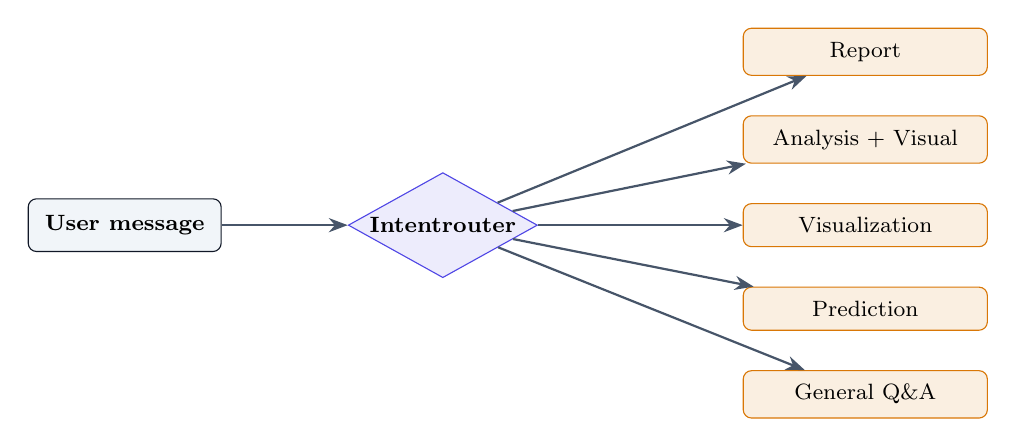
\begin{tikzpicture}[node distance=5mm and 16mm,
  q/.style={draw=uaInk,fill=uaMist,rounded corners=3pt,font=\footnotesize\bfseries,inner sep=6pt},
  r/.style={diamond,draw=uaIndigo,fill=uaIndigo!10,aspect=1.8,font=\footnotesize\bfseries,inner sep=1pt},
  s/.style={draw=uaAmber,fill=uaAmber!12,rounded corners=3pt,font=\footnotesize,inner sep=5pt,minimum width=3.1cm},
  a/.style={-{Stealth[length=2.4mm]},uaSlate,thick,font=\scriptsize}]
  \node[q] (msg) {User message};
  \node[r,right=of msg] (rt) {Intent\\router};
  \node[s,right=26mm of rt] (viz) {Visualization};
  \node[s,above=of viz] (av) {Analysis + Visual};
  \node[s,above=of av] (rep) {Report};
  \node[s,below=of viz] (pred) {Prediction};
  \node[s,below=of pred] (qa) {General Q\&A};

  \draw[a] (msg) -- (rt);
  \draw[a] (rt) -- (rep);
  \draw[a] (rt) -- (av);
  \draw[a] (rt) -- (viz);
  \draw[a] (rt) -- (pred);
  \draw[a] (rt) -- (qa);
\end{tikzpicture}
\caption{Intent routing. Higher-signal intents (report, prediction, dashboard)
are detected first; everything else falls through to grounded Q\&A.}
\label{fig:router}
\end{figure}

\begin{lstlisting}[style=py,caption={The heuristic skill selector (\code{\_select\_skill}).}]
def _select_skill(message: str) -> str:
    if _is_report_request(message):
        return SKILL_REPORT
    if _is_prediction_request(message):
        return SKILL_PREDICTION
    if _is_dashboard_request(message):
        return SKILL_ANALYSIS_WITH_VISUAL
    # ... visualization vs analysis heuristics ...
    if <visual intent>:
        return SKILL_VISUALIZATION
    return SKILL_GENERAL_QA
\end{lstlisting}

\section{The skill registry}
Each skill has a Markdown definition in \code{app/skills\_registry/}. These files
are not code --- they are \emph{instructions to the model}, loaded at request
time and injected into the prompt as skill guidelines. Keeping them as editable
Markdown means the team can tune model behaviour per skill without touching
Python.

\begin{table}[h]
\centering
\caption{Skills, their registry files, and behaviour.}
\small
\begin{tabularx}{\linewidth}{@{}L{2.5cm} L{2.6cm} X@{}}
\toprule
\textbf{Skill} & \textbf{Registry file} & \textbf{Behaviour} \\
\midrule
Analysis & \code{analysis.md} & Grounded statistical analysis over the profile
and retrieved context. \\
Visualization & \code{visualization.md} & Plans a strict chart specification
that is validated and rendered. \\
Analysis + Visual & \code{analysis.md} + \code{visualization.md} & A dashboard
request: prose analysis plus one or more charts. \\
Cleaning & \code{cleaning.md} & Guided cleaning with transparent, listed
actions. \\
Prediction & \code{prediction.md} & Target selection, model choice, training,
evaluation. \\
Report & \code{report.md} & Assembles the branded PDF report. \\
General Q\&A & \code{general\_qa.md} & Open questions grounded in retrieval. \\
\bottomrule
\end{tabularx}
\end{table}

\section{Prompt composition}
The chat handler composes the final prompt from three parts: a base prompt
(profile summary plus grounded context), the selected skill's guidelines, and a
turn instruction. Composition is skill-aware. For a visualization turn, the
model is steered toward emitting a structured chart plan; for prose skills, the
handler appends an explicit instruction that the model must \emph{not} emit JSON
or code blocks --- only clean prose --- so the answer renders cleanly in the
chat surface.

\begin{lstlisting}[style=py,caption={Prose skills forbid code/JSON output to keep answers clean.}]
return (f"{base_prompt}\n\n## AI SKILL GUIDELINES\n{skill_text}"
        f"\n\n## TURN INSTRUCTION\n{instruction}\n"
        "CRITICAL: You MUST NOT output any JSON, code blocks, or python code. "
        "Output only clean prose. Do not start any markdown code blocks.")
\end{lstlisting}

\section{Thinking mode}
For questions that warrant it, the system can request an intermediate
\emph{thinking} pass, surfaced to the user as a distinct \code{thinking} event
rather than mixed into the answer. This keeps the visible answer crisp while
still exposing the model's reasoning for users who want it --- consistent with
the product's preference for exactness over theatrics.

\section{Skill outputs and UI commands}
Skills do more than produce text. A dashboard turn emits a \code{command} event
that switches the interface to the dashboard view and a \code{chart} event for
each validated figure. A report turn emits a \code{download\_report} command.
This command channel lets the backend drive the front-end experience without the
front end having to infer intent from prose --- the routing decision made on the
server is communicated explicitly to the client.

\begin{uanote}[Registry as a tuning surface]
Because skill behaviour lives in Markdown, iterating on how the model analyses,
visualizes, or cleans data is a documentation edit --- reviewable in a pull
request --- rather than a code change. This cleanly separates \emph{prompt
engineering} from \emph{application logic}.
\end{uanote}

%=============================================================================
%  09_visualization.tex  -  Chapter 8: The Visualization Engine
%=============================================================================
\chapter{The Visualization Engine}
\label{ch:viz}

Charts are where a hallucinating assistant does the most damage, so this is
where Universal Analyst is strictest. The model never draws anything. It emits a
\emph{plan}; the backend validates that plan against the real schema and only
then renders a Plotly figure. This chapter covers the chart-type catalogue, the
plan schema, and the validation-and-render pipeline in \code{ChartFactory}.

\section{A broad chart catalogue}
The \code{ChartType} enumeration defines the full set of visualizations the
system understands --- twenty-six types spanning statistical, hierarchical,
geographic, and multidimensional charts. The enum is the single source of truth:
the plan schema references it, and the factory validates against it.

\begin{table}[h]
\centering
\caption{The \code{ChartType} catalogue (26 types).}
\small
\begin{tabularx}{\linewidth}{@{}L{2.6cm} X@{}}
\toprule
\textbf{Family} & \textbf{Types} \\
\midrule
Comparison & \code{bar}, \code{line}, \code{area}, \code{funnel},
\code{funnel\_area}, \code{waterfall} \\
Distribution & \code{histogram}, \code{box}, \code{violin}, \code{strip},
\code{density\_heatmap}, \code{density\_contour} \\
Relationship & \code{scatter}, \code{heatmap}, \code{scatter\_matrix},
\code{scatter\_3d} \\
Composition & \code{pie}, \code{treemap}, \code{sunburst}, \code{icicle} \\
Multidimensional & \code{radar}, \code{parallel\_coordinates},
\code{parallel\_categories} \\
Geographic & \code{scatter\_geo}, \code{choropleth} \\
Indicator & \code{gauge}, \code{timeline} \\
\bottomrule
\end{tabularx}
\end{table}

\section{The chart plan}
When a visualization is requested, the model is asked to emit a structured chart
\emph{plan} rather than any drawing code. The plan is constrained by a
JSON schema generated at request time from the actual column names, so the model
can only reference columns that exist. Ollama's structured-output mode
(Chapter~\ref{ch:llm}) is used to force schema-valid output where supported.

\begin{figure}[h]
\centering
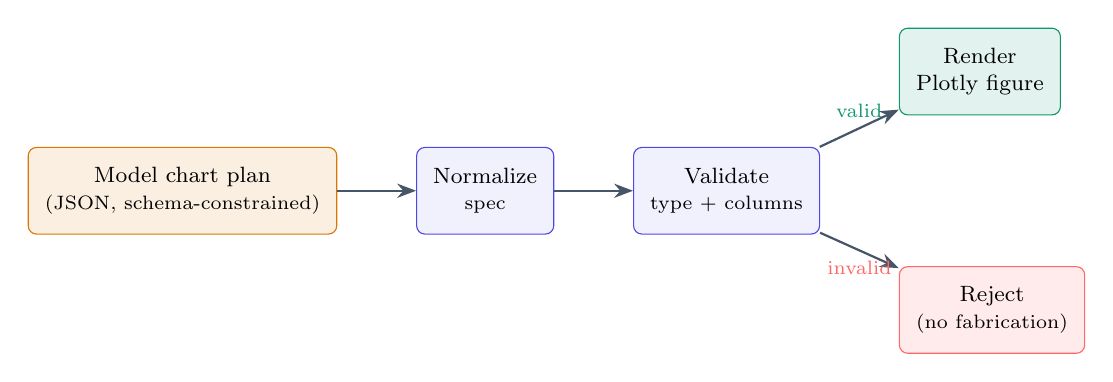
\begin{tikzpicture}[node distance=6mm and 10mm,
  b/.style={draw,rounded corners=3pt,align=center,font=\footnotesize,inner sep=6pt,minimum height=11mm},
  m/.style={b,draw=uaAmber,fill=uaAmber!12},
  v/.style={b,draw=uaIndigo,fill=uaIndigo!8},
  ok/.style={b,draw=uaGreen,fill=uaGreen!12},
  no/.style={b,draw=red!60,fill=red!8},
  a/.style={-{Stealth[length=2.4mm]},uaSlate,thick,font=\scriptsize}]
  \node[m] (plan) {Model chart plan\\\scriptsize (JSON, schema-constrained)};
  \node[v,right=of plan] (norm) {Normalize\\\scriptsize spec};
  \node[v,right=of norm] (val) {Validate\\\scriptsize type + columns};
  \node[ok,above right=4mm and 10mm of val] (render) {Render\\Plotly figure};
  \node[no,below right=4mm and 10mm of val] (reject) {Reject\\\scriptsize (no fabrication)};
  \draw[a] (plan) -- (norm);
  \draw[a] (norm) -- (val);
  \draw[a] (val) -- node[above,font=\scriptsize,text=uaGreen]{valid} (render);
  \draw[a] (val) -- node[below,font=\scriptsize,text=red!60]{invalid} (reject);
\end{tikzpicture}
\caption{The validation-first visualization pipeline. Invalid plans are
rejected, never silently replaced with a placeholder chart.}
\label{fig:chartpipe}
\end{figure}

\section{The chart factory}
\code{ChartFactory.generate\_chart} takes the DataFrame and a normalized chart
specification and produces a rendered figure. Before any rendering it performs a
battery of checks:

\begin{itemize}
  \item The requested type must be a member of \code{ChartType}.
  \item Every referenced column must actually exist in the DataFrame
        (a \code{\_valid} predicate).
  \item Columns used on numeric axes must genuinely be numeric
        (a \code{\_is\_numeric} predicate).
  \item Optional filters are applied through a dedicated \code{\_apply\_filters}
        step before aggregation.
\end{itemize}

Only after these pass does the factory aggregate, optionally take a top-$N$
slice for categorical charts, apply a consistent aesthetic, and hand off to
Plotly. A plan that references a missing column, or asks for a numeric axis on a
categorical field, does not produce a degraded chart --- it fails validation.

\begin{lstlisting}[style=py,caption={Validation predicates inside \code{ChartFactory.generate\_chart}.}]
supported_types = {t.value for t in ChartType}
# ...
def _valid(col):
    return col is not None and col in df.columns
def _is_numeric(col):
    return _valid(col) and pd.api.types.is_numeric_dtype(df[col])
\end{lstlisting}

\section{Consistent aesthetics}
A single \code{\_apply\_aesthetic} routine styles every figure so that charts
generated across a session read as one product: shared fonts, restrained
gridlines, and the indigo/amber signature rather than Plotly's defaults. This is
the visual analogue of the ``one signal, one job'' principle --- colour carries
meaning, not decoration.

\section{From plan to dashboard}
A dashboard request can yield multiple charts. Each validated figure is stored
on the session (so it can later appear in the PDF report) and streamed to the
front end as a \code{chart} event, while a \code{command} event switches the UI
to the dashboard view. Chart titles are extracted from the specification, with a
sensible fallback, so every tile is labelled.

\begin{uawarn}[Validation is the product]
It would be easy --- and tempting --- to ``fix up'' a slightly wrong plan or
fall back to a default chart when validation fails. The system does neither. A
chart that cannot be built correctly from the real data is not built. This is
the visualization-layer expression of the no-fabrication rule.
\end{uawarn}

\section{Direct visualization endpoint}
Beyond model-driven dashboards, the \code{/visualize} endpoint accepts an
explicit, already-validated chart specification and returns a rendered figure.
This gives the front end a deterministic path for user-initiated charts that do
not require the model at all, reusing the very same factory and therefore the
very same validation guarantees.

%=============================================================================
%  10_prediction.tex  -  Chapter 9: The Prediction Engine
%=============================================================================
\chapter{The Prediction Engine}
\label{ch:predict}

The prediction skill lets an analyst go beyond description into lightweight
modelling: ``can this dataset predict X?'' It is a hybrid pipeline --- the
language model reasons about \emph{what} to model and \emph{which} algorithm to
use, while scikit-learn does the actual training and evaluation. The model
advises; deterministic code decides and measures.

\section{Pipeline stages}
\begin{figure}[h]
\centering
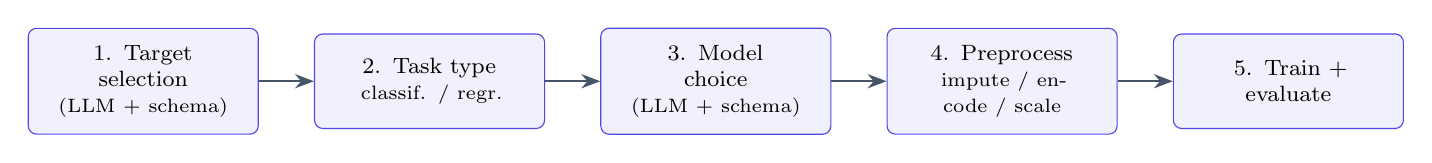
\begin{tikzpicture}[node distance=4mm and 7mm,
  s/.style={draw=uaIndigo,fill=uaIndigo!8,rounded corners=3pt,align=center,
    font=\footnotesize,inner sep=6pt,minimum height=12mm,text width=2.5cm},
  a/.style={-{Stealth[length=2.4mm]},uaSlate,thick}]
  \node[s] (t) {1. Target\\selection\\\scriptsize (LLM + schema)};
  \node[s,right=of t] (k) {2. Task type\\\scriptsize classif. / regr.};
  \node[s,right=of k] (m) {3. Model\\choice\\\scriptsize (LLM + schema)};
  \node[s,right=of m] (p) {4. Preprocess\\\scriptsize impute / encode / scale};
  \node[s,right=of p] (e) {5. Train +\\evaluate};
  \draw[a](t)--(k); \draw[a](k)--(m); \draw[a](m)--(p); \draw[a](p)--(e);
\end{tikzpicture}
\caption{The five-stage prediction pipeline, blending LLM reasoning (stages 1--3)
with scikit-learn execution (stages 4--5).}
\label{fig:predict}
\end{figure}

\section{Target and task selection}
The first decision --- which column to predict --- is made by the model, but
inside a schema. A generated JSON schema constrains the model to choose a
\code{target\_column} from the real column list, give a \code{reason}, and
declare the \code{task\_type} as either \code{classification} or
\code{regression}. Structured output turns this from a free-text guess into a
validated selection.

\begin{lstlisting}[style=py,caption={The target-selection schema (abridged).}]
{
  "target_column": {"type": "string", "enum": columns},
  "reason": {"type": "string"},
  "task_type": {"type": "string", "enum": ["classification", "regression"]}
}  # required: target_column, reason, task_type
\end{lstlisting}

\section{Model selection}
Given the task type, a second schema constrains the model to pick an appropriate
scikit-learn algorithm and its hyperparameters from a curated list. Offering the
model a fixed menu --- rather than free choice --- guarantees that whatever it
returns can actually be instantiated and trained.

\begin{table}[h]
\centering
\caption{Candidate models offered to the LLM per task type.}
\small
\begin{tabularx}{\linewidth}{@{}L{3.0cm} X@{}}
\toprule
\textbf{Task} & \textbf{Candidate estimators} \\
\midrule
Classification & \code{logistic\_regression}, \code{random\_forest\_classifier},
\code{gradient\_boosting\_classifier}, \code{decision\_tree\_classifier},
\code{svm\_classifier}, \code{knn\_classifier} \\
Regression & \code{linear\_regression}, \code{ridge}, \code{lasso},
\code{random\_forest\_regressor}, \code{gradient\_boosting\_regressor},
\code{decision\_tree\_regressor}, \code{svr}, \code{knn\_regressor} \\
\bottomrule
\end{tabularx}
\end{table}

\section{Preprocessing}
Before training, the pipeline prepares features deterministically with
scikit-learn utilities: missing values are imputed (\code{SimpleImputer}),
categorical features are label-encoded (\code{LabelEncoder}), and numeric
features are standardized (\code{StandardScaler}). The data is split into train
and test partitions with \code{train\_test\_split}. None of this touches the
language model --- it is ordinary, reproducible feature engineering.

\begin{lstlisting}[style=py,caption={The scikit-learn building blocks used by the pipeline.}]
from sklearn.model_selection import train_test_split
from sklearn.preprocessing import LabelEncoder, StandardScaler
from sklearn.impute import SimpleImputer
from sklearn.linear_model import LogisticRegression, LinearRegression, Ridge, Lasso
from sklearn.ensemble import (RandomForestClassifier, RandomForestRegressor,
                              GradientBoostingClassifier, GradientBoostingRegressor)
from sklearn.tree import DecisionTreeClassifier, DecisionTreeRegressor
from sklearn.svm import SVC, SVR
from sklearn.neighbors import KNeighborsClassifier, KNeighborsRegressor
\end{lstlisting}

\section{Training and evaluation}
The chosen estimator is fit on the training partition and evaluated on the held-
out test set with task-appropriate metrics: accuracy, precision, recall, F1, and
a classification report for classification; $R^2$ and error metrics for
regression. The results --- the selected target and its rationale, the chosen
model, and the metrics --- are streamed back so the user sees not just a number
but \emph{why} this model was chosen and how well it did.

\begin{table}[h]
\centering
\caption{Evaluation metrics by task type.}
\small
\begin{tabularx}{\linewidth}{@{}L{3.0cm} X@{}}
\toprule
\textbf{Task} & \textbf{Metrics reported} \\
\midrule
Classification & Accuracy, precision, recall, F1, and a full classification
report. \\
Regression & $R^2$ score and error measures. \\
\bottomrule
\end{tabularx}
\end{table}

\begin{uanote}[Bounded autonomy]
The model is given real agency --- it selects the target and the algorithm ---
but only within schemas and a fixed estimator menu. This is the project's
signature pattern applied to machine learning: \emph{the model proposes within a
contract; deterministic code disposes and measures.}
\end{uanote}

%=============================================================================
%  11_reporting.tex  -  Chapter 10: Cleaning and PDF Reporting
%=============================================================================
\chapter{Cleaning and PDF Reporting}
\label{ch:reporting}

Two skills turn analysis into deliverables: the cleaning skill, which produces a
tidier dataset with a transparent record of what changed, and the report skill,
which exports a branded PDF capturing the whole session. Both are held to the
same honesty standard as the rest of the system.

\section{The cleaning skill}
The cleaning skill applies guided data-cleaning operations to a session's
DataFrame and returns a structured \code{CleaningResponse}. Critically, it does
not clean silently: the response enumerates exactly what happened.

\begin{table}[h]
\centering
\caption{Fields of \code{CleaningResponse}.}
\small
\begin{tabularx}{\linewidth}{@{}L{3.6cm} X@{}}
\toprule
\textbf{Field} & \textbf{Meaning} \\
\midrule
\code{original\_rows} / \code{cleaned\_rows} & Row counts before and after. \\
\code{original\_columns} / \code{cleaned\_columns} & Column counts before and
after. \\
\code{actions} & An ordered list of the cleaning operations performed. \\
\code{explanation} & A human-readable rationale for the changes. \\
\code{profile} & A fresh \code{DataProfile} of the cleaned data. \\
\code{preview\_rows} & A sample of the cleaned rows for immediate inspection. \\
\bottomrule
\end{tabularx}
\end{table}

Because the response includes a fresh profile and a preview, the front end can
show the effect of cleaning immediately, and the user can decide whether to keep
the result --- optionally as a new session, via the
\code{create\_new\_session} flag on the request. Transparency here is the point:
an analyst must be able to see and justify every transformation applied to their
data.

\begin{uanote}[Cleaning is auditable]
Every cleaning run returns the list of actions taken and a before/after profile.
There is no ``magic tidy'' that changes the data without saying how --- the
transformation is as inspectable as the analysis.
\end{uanote}

\section{The report skill}
The report skill produces a professional, branded PDF using \textbf{ReportLab}.
It is deliberately designed so that ``the PDF and the app read as one product'':
the same indigo/amber identity, the same monospaced treatment of numbers, and
the same restraint.

\subsection{Document structure}
A report is assembled with ReportLab's \code{platypus} flowable system on A4
pages. A custom stylesheet defines a coherent hierarchy --- title, subtitle,
eyebrow, headings, body, muted, and small styles --- so the document has
deliberate typographic rhythm rather than default styling.

\begin{table}[h]
\centering
\caption{Sections composed into the PDF report.}
\small
\begin{tabularx}{\linewidth}{@{}L{3.4cm} X@{}}
\toprule
\textbf{Section} & \textbf{Content} \\
\midrule
Cover / header & Branded title block establishing the report identity. \\
Data profile & Row/column counts, per-column types, and key statistics. \\
Quality signals & Missingness, outliers, and other profile-derived signals. \\
Generated charts & The validated charts produced during the session. \\
Narrative & A model-written summary from the report-narrative generator. \\
Transcript & The conversation that produced the analysis. \\
\bottomrule
\end{tabularx}
\end{table}

\subsection{Embedding real charts}
The charts in the report are the very same validated figures generated during
the session --- not re-imagined for print. Plotly figures are rasterized to
images through \textbf{Kaleido} and embedded into the PDF, so what the analyst
saw on screen is what appears in the document. This closes the loop: a chart
that passed validation in the dashboard is the chart that lands in the report.

\subsection{The report narrative}
A dedicated \code{report\_narrative} generator asks the model for a concise,
prose summary of the findings, which is embedded as the narrative section. It
uses the non-streaming \code{generate\_text} path (Chapter~\ref{ch:llm}), so a
model failure raises rather than silently producing an empty section --- once
again, no fabrication.

\begin{lstlisting}[style=py,caption={ReportLab flowables used to build the document.}]
from reportlab.lib.pagesizes import A4
from reportlab.lib.styles import ParagraphStyle, getSampleStyleSheet
from reportlab.platypus import (SimpleDocTemplate, Paragraph, Spacer,
                                Table, TableStyle, Image)
# A custom stylesheet (title/subtitle/eyebrow/h1/h2/body/muted/small)
# gives the PDF the same visual identity as the application.
\end{lstlisting}

\subsection{Robust value formatting}
Report generation is defensive about the messy reality of real data. Helper
routines (\code{\_fmt}, \code{\_plain}, \code{\_safe\_text},
\code{\_inline\_markdown}, \code{\_top\_value\_text}) coerce arbitrary profile
values into clean, length-bounded strings, strip inline Markdown, and format
top-value lists --- so a stray \code{NaN}, an over-long category label, or an
exotic type never breaks the layout.

\section{Delivery}
The report is requested through \code{POST /skills/report}. In the chat flow, a
report intent additionally emits a \code{download\_report} command event so the
front end can trigger the download as part of the conversation, making export
feel like a natural continuation of the analysis rather than a separate mode.

%=============================================================================
%  12_frontend.tex  -  Chapter 11: The Front End
%=============================================================================
\chapter{The Front End}
\label{ch:frontend}

The interface is a React\,18 single-page application built with Vite and styled
with TailwindCSS. It is deliberately thin: all intelligence lives in the
backend, and the front end's job is to present streamed results faithfully,
enforce the product's visual discipline, and stay out of the analyst's way.

\section{Application shell}
The app is organized around four tabs --- \textbf{Profile}, \textbf{Dashboard},
\textbf{Chat}, and \textbf{Prediction} --- with a session sidebar, a command
palette, and a chart gallery layered on top. State for the active session,
profile, EDA, charts, dashboard layout, and composer draft is held at the app
root and threaded to components.

\begin{lstlisting}[style=js,caption={The four primary views.}]
const TABS = { PROFILE: 'profile', DASHBOARD: 'dashboard',
               CHAT: 'chat', PREDICTION: 'prediction' };
\end{lstlisting}

\begin{table}[h]
\centering
\caption{Key front-end components and their roles.}
\small
\begin{tabularx}{\linewidth}{@{}L{3.5cm} X@{}}
\toprule
\textbf{Component} & \textbf{Role} \\
\midrule
\code{FileUpload} & Drag-and-drop intake; posts to \code{/upload}. \\
\code{DataOverview} & Renders the profile and EDA panels. \\
\code{ChatInput} / \code{ChatMessage} & Composer (text, images, voice) and
message rendering. \\
\code{MessageList} & The streamed conversation. \\
\code{DashboardGrid} / \code{ChartCard} & Model-generated dashboard tiles. \\
\code{LazyChartCard} & Defers the heavy Plotly bundle until a chart is shown. \\
\code{PredictionPanel} & Drives and displays the prediction skill. \\
\code{SessionSidebar} & Session list and switching. \\
\code{CommandPalette} & Keyboard-driven actions. \\
\code{ContextRing} & Visual token-usage meter. \\
\code{ReportButton} & Triggers PDF export. \\
\bottomrule
\end{tabularx}
\end{table}

\section{Consuming the event stream}
The \code{useChat} hook is the heart of the client. It issues a \code{fetch} to
\code{/chat}, reads the response body as a stream, and decodes Server-Sent
Events incrementally with a \code{TextDecoder}, dispatching on the event name to
patch the in-progress assistant message. Tokens append live, \code{thinking}
renders as a distinct affordance, \code{chart} events populate the dashboard,
\code{usage} updates the meter, and \code{command} events drive view changes.

\begin{lstlisting}[style=js,caption={Incremental SSE decoding in \code{useChat}.}]
const reader = response.body.getReader();
const decoder = new TextDecoder();
// ... read loop ...
const { done, value } = await reader.read();
buffer += decoder.decode(value, { stream: true });
// parse lines: `event: <name>` then `data: <json>`; switch on eventName
\end{lstlisting}

Two supporting hooks round out data flow: \code{useFileUpload} manages the
intake request and its progress, and \code{useSessions} lists, selects, and
deletes sessions against the \code{/sessions} endpoints.

\section{Multimodal and voice input}
The composer accepts image attachments, enforcing the backend-advertised limits
(count and size) before send, and base64-encodes them for the multimodal path.
It also offers optional browser speech-to-text: dictated text is inserted into
the composer as an \emph{enhancement}, never as the only input path --- honouring
the accessibility principle from Chapter~\ref{ch:product}.

\section{Performance: lazy Plotly}
Plotly is by far the heaviest dependency (roughly 3\,MB). The Vite build splits
it, along with the Markdown renderer and core vendor libraries, into separate
chunks via \code{manualChunks}, and the \code{LazyChartCard} component defers
loading the Plotly bundle until a chart actually needs to render. The result is
that the intake and profile views paint quickly; the visualization cost is paid
only when the analyst asks for a chart.

\begin{lstlisting}[style=js,caption={Manual chunking keeps the initial bundle small.}]
manualChunks: {
  plotly:   ['plotly.js-dist-min', 'react-plotly.js'],
  markdown: ['react-markdown', 'remark-gfm'],
  vendor:   ['react', 'react-dom', 'lucide-react'],
}
\end{lstlisting}

\section{The \code{/api} proxy}
The front end always calls \code{/api/*}. In development, Vite's proxy forwards
those calls to the backend on port 8000 and strips the \code{/api} prefix; the
built assets use a relative base so the notebook can serve \code{dist/} from any
sub-path, and in production a reverse proxy maps \code{/api} to the backend. The
client code is identical in every environment.

\section{Robustness and feedback}
An \code{ErrorBoundary} contains rendering failures so a single bad chart cannot
blank the whole app, a \code{Toast} surfaces transient notifications, and a
\code{LoadingBar} communicates in-flight work. Together with the token meter,
these give the analyst continuous, honest feedback about what the system is
doing --- the interface-level counterpart to the backend's no-fabrication rule.

\begin{uanote}[Thin client, exact readouts]
The front end renders numbers in IBM Plex Mono, defers heavy work, and shows
real streamed state --- reasoning, tokens, usage, errors --- exactly as the
backend reports it. It presents the instrument; it does not invent readings.
\end{uanote}

%=============================================================================
%  13_api.tex  -  Chapter 12: The HTTP API
%=============================================================================
\chapter{The HTTP API}
\label{ch:api}

The backend exposes a compact REST surface. All routes are served at the root of
port \code{8000} and reached by the front end through the \code{/api} proxy. This
chapter enumerates the endpoints, groups them by concern, and details the two
most important flows.

\section{Endpoint catalogue}
\begin{table}[h]
\centering
\caption{Complete endpoint listing, grouped by router tag.}
\small
\begin{tabularx}{\linewidth}{@{}l L{3.6cm} X@{}}
\toprule
\textbf{Method} & \textbf{Path} & \textbf{Description} \\
\midrule
\code{GET} & \code{/health} & Liveness check. \\
\code{GET} & \code{/capabilities} & Feature metadata (image limits, flags). \\
\midrule
\code{POST} & \code{/upload} & Ingest a file; returns \code{session\_id},
\code{profile}, \code{eda}. \\
\midrule
\code{POST} & \code{/chat} & Streamed chat (SSE event protocol). \\
\midrule
\code{POST} & \code{/visualize} & Render a Plotly chart from a validated spec. \\
\midrule
\code{POST} & \code{/clean} & Guided data cleaning; returns
\code{CleaningResponse}. \\
\midrule
\code{POST} & \code{/predict} & Run the prediction pipeline. \\
\midrule
\code{GET} & \code{/sessions} & List sessions with counts. \\
\code{POST} & \code{/sessions} & Create a session. \\
\code{GET} & \code{/sessions/\{id\}} & Session details, history, charts. \\
\code{DELETE} & \code{/sessions/\{id\}} & Delete a session and its collection. \\
\midrule
\code{GET} & \code{/skills} & Active skill manifest. \\
\code{POST} & \code{/skills/report} & Generate a PDF report. \\
\bottomrule
\end{tabularx}
\end{table}

\section{Router composition}
Routes are assembled from per-concern routers into one \code{api\_router}, each
tagged for the automatically generated OpenAPI documentation available at
\code{/docs}. The skills router is mounted under a \code{/skills} prefix; all
others sit at the root.

\begin{lstlisting}[style=py,caption={Router composition (\code{app/api/router.py}).}]
api_router.include_router(health.router, tags=["health"])
api_router.include_router(upload.router, tags=["upload"])
api_router.include_router(chat.router, tags=["chat"])
api_router.include_router(visualizations.router, tags=["visualizations"])
api_router.include_router(sessions.router, tags=["sessions"])
api_router.include_router(skills_api.router, prefix="/skills", tags=["skills"])
api_router.include_router(clean.router, tags=["clean"])
api_router.include_router(predict.router, tags=["prediction"])
\end{lstlisting}

\section{The upload flow}
\code{POST /upload} is the entry point of every session. It accepts a
multipart file, parses it with the \code{IngestionEngine}, profiles it with the
\code{DataProfiler}, runs auto-EDA, chunks and embeds the data into a new
ChromaDB collection, and returns a \code{session\_id} together with the profile
and EDA payloads. From that point on the \code{session\_id} identifies the
dataset for every subsequent call.

\begin{table}[h]
\centering
\caption{\code{/upload} response payload.}
\small
\begin{tabularx}{\linewidth}{@{}L{3.0cm} X@{}}
\toprule
\textbf{Field} & \textbf{Content} \\
\midrule
\code{session\_id} & UUID identifying the new session. \\
\code{profile} & The full \code{DataProfile} (types, statistics, correlations). \\
\code{eda} & The automated exploratory-analysis summary. \\
\bottomrule
\end{tabularx}
\end{table}

\section{The chat flow}
\code{POST /chat} is the richest endpoint. It accepts the session id, the user
message, optional image attachments, and flags such as thinking mode. It routes
the message to a skill, builds a grounded prompt, streams the model's output,
validates and renders any requested charts, accounts for token usage, persists
the exchange to the session, and emits UI commands --- all as a single SSE
stream using the event protocol of Table~\ref{tab:events}.

\section{CORS and configuration}
Cross-origin behaviour is driven by \code{ALLOWED\_ORIGINS}. When a wildcard is
configured the app switches to an origin-regex policy \emph{without} credentials
(the specification forbids credentials with a wildcard origin); otherwise it
allows the listed origins \emph{with} credentials. This detail matters for
correct, secure browser access across the different deployment topologies.

\begin{lstlisting}[style=py,caption={Credential-safe CORS handling in \code{main.py}.}]
if "*" in _origins:
    app.add_middleware(CORSMiddleware, allow_origin_regex=".*",
        allow_credentials=False, allow_methods=["*"], allow_headers=["*"])
else:
    app.add_middleware(CORSMiddleware, allow_origins=_origins,
        allow_credentials=True, allow_methods=["*"], allow_headers=["*"])
\end{lstlisting}

\begin{uanote}[Self-documenting API]
Because the backend is FastAPI, the endpoint catalogue above is also available
as live, interactive OpenAPI documentation at \code{/docs} --- useful during
development and for graders exploring the running service.
\end{uanote}

%=============================================================================
%  14_deployment.tex  -  Chapter 13: Configuration and Deployment
%=============================================================================
\chapter{Configuration and Deployment}
\label{ch:deploy}

Universal Analyst is designed to run on a cloud GPU box with the language model
local to the machine, and to be brought up with a single notebook or a single
\code{make} command. This chapter covers configuration, the three deployment
shapes, and the developer tooling.

\section{Configuration}
All settings are read through \code{pydantic-settings} from environment
variables (or a \code{.env} file), with sensible defaults and alias support so
the same setting can be spelled several ways. Table~\ref{tab:env} lists the
important keys; the full template ships as \code{.env.example} and is reproduced
in Appendix~\ref{app:env}.

\begin{table}[h]
\centering
\caption{Principal configuration variables.}
\label{tab:env}
\small
\begin{tabularx}{\linewidth}{@{}L{4.3cm} L{3.0cm} X@{}}
\toprule
\textbf{Variable} & \textbf{Default} & \textbf{Purpose} \\
\midrule
\code{OLLAMA\_HOST} & \code{localhost:11434} & Ollama runtime URL. \\
\code{MODEL\_NAME} & \code{gemma4:12b} & Primary answering model. \\
\code{ROUTER\_MODEL\_NAME} & \code{gemma4:e4b} & Fast routing model. \\
\code{EMBEDDING\_MODEL} & \code{all-MiniLM-L6-v2} & RAG embeddings. \\
\code{MAX\_CONTEXT\_TOKENS} & \code{6000} & RAG context budget. \\
\code{CONTEXT\_WINDOW\_TOKENS} & \code{256000} & Front-end meter window. \\
\code{IMAGE\_CHAT\_ENABLED} & \code{true} & Multimodal image path. \\
\code{MAX\_CHAT\_IMAGES} & \code{3} & Images per turn. \\
\code{MAX\_CHAT\_IMAGE\_MB} & \code{5} & Size per image. \\
\code{CHROMA\_PERSIST\_DIRECTORY} & \code{./chroma\_data} & Vector-store path. \\
\code{ALLOWED\_ORIGINS} & \code{localhost:5173,...} & CORS allowlist. \\
\bottomrule
\end{tabularx}
\end{table}

\begin{lstlisting}[style=py,caption={Settings with multi-alias support (\code{app/config.py}).}]
class Settings(BaseSettings):
    model_name: str = "gemma4:12b"
    router_model_name: str = "gemma4:e4b"
    embedding_model: str = "all-MiniLM-L6-v2"
    max_context_tokens: int = 6000
    environment: str = Field(default="development",
        validation_alias=AliasChoices("ENVIRONMENT", "ENV", "environment", "env"))
    # ... image limits, chroma dir, allowed_origins ...
    model_config = SettingsConfigDict(env_file=".env", extra="ignore",
                                      populate_by_name=True)
\end{lstlisting}

\section{Cloud notebook setup}
The primary path for graders and cloud users is \code{main.ipynb}. Running all
cells installs dependencies idempotently, pulls the required Gemma tags
(\code{gemma4:12b} and \code{gemma4:e4b}), and starts both services. If a
required model tag is unavailable, setup \emph{stops with a real error} rather
than degrading silently --- so the runtime can be fixed directly. The forwarded
port 5173 serves the app and 8000 exposes the API docs.

\section{Docker Compose}
Two compose files cover development and production.

\begin{description}[style=nextline,leftmargin=0pt]
  \item[\textcolor{uaIndigoD}{Development (\code{docker-compose.yml})}]
    Bind-mounts the backend and frontend source for live reload, runs the Vite
    dev server directly from a Node image (so hot-module reload and the
    \code{/api} proxy work out of the box), and reaches an Ollama running on the
    host via \code{host.docker.internal}.
  \item[\textcolor{uaIndigoD}{Production (\code{docker-compose.prod.yml})}]
    Builds optimized images and serves the front end's static assets behind
    nginx, which also proxies \code{/api} to the backend.
\end{description}

\begin{lstlisting}[style=bash,caption={Developer entry points via the Makefile.}]
make up          # dev: backend :8000 + Vite dev server :5173 (Ollama on host)
make prod-up     # prod: built images behind nginx
make down        # stop
make logs        # follow logs
make test        # backend pytest
make lint        # ruff check
make format      # ruff format
\end{lstlisting}

\section{Container images}
The backend \code{Dockerfile} builds a Python\,3.12 service image; the frontend
\code{Dockerfile} builds the production nginx image serving the compiled SPA. The
Makefile detects Docker Compose v2 (\code{docker compose}) and falls back to the
legacy v1 binary if only that is present, so the same commands work across
environments.

\section{Manual startup}
For a bare host, the sequence is: pull the models
(\code{scripts/setup\_ollama.sh}), install backend requirements and launch
\code{uvicorn} on port 8000, then install and run the Vite dev server. Copying
\code{.env.example} to \code{.env} configures models, the Ollama host, the RAG
budget, and CORS.

\begin{lstlisting}[style=bash,caption={Manual startup on a bare GPU host.}]
bash scripts/setup_ollama.sh
cd backend && pip install -r requirements.txt
uvicorn app.main:app --host 0.0.0.0 --port 8000
cd ../frontend && npm install && npm run dev -- --host
\end{lstlisting}

\begin{uawarn}[Ollama placement matters]
Under Docker, the backend reaches Ollama on the \emph{host} through
\code{host.docker.internal}, not \code{localhost}. Getting this wrong is the most
common local-setup mistake; the environment template documents both forms.
\end{uawarn}

%=============================================================================
%  15_testing.tex  -  Chapter 14: Testing and Quality
%=============================================================================
\chapter{Testing and Quality Assurance}
\label{ch:testing}

Quality is enforced continuously rather than inspected at the end. Every push and
pull request to \code{main} triggers a two-job pipeline that lints and tests the
backend and builds the front end, so a change that breaks either half cannot
merge unnoticed.

\section{Continuous integration}
The GitHub Actions workflow defines two parallel jobs
(Figure~\ref{fig:ci}): \code{backend-tests} and \code{frontend-build}.

\begin{figure}[h]
\centering
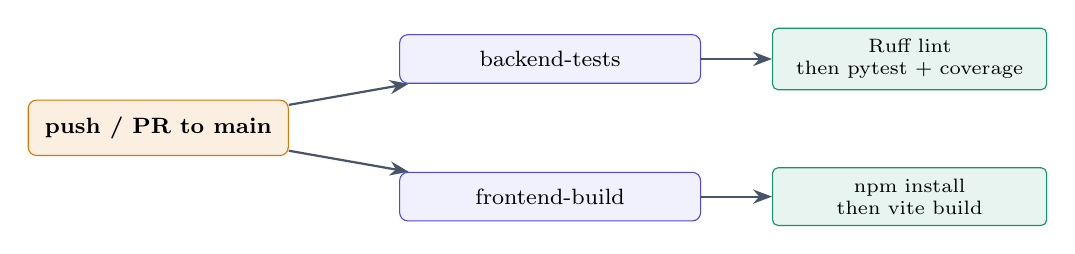
\begin{tikzpicture}[node distance=4mm and 9mm,
  ev/.style={draw=uaAmber,fill=uaAmber!12,rounded corners=3pt,font=\footnotesize\bfseries,inner sep=6pt},
  j/.style={draw=uaIndigo,fill=uaIndigo!8,rounded corners=3pt,font=\footnotesize,inner sep=6pt,text width=3.4cm,align=center},
  st/.style={draw=uaGreen,fill=uaGreen!10,rounded corners=2pt,font=\scriptsize,inner sep=4pt,text width=3.2cm,align=center},
  a/.style={-{Stealth[length=2.4mm]},uaSlate,thick}]
  \node[ev] (push) {push / PR to main};
  \node[j,above right=2mm and 14mm of push] (be) {backend-tests};
  \node[j,below right=2mm and 14mm of push] (fe) {frontend-build};
  \node[st,right=of be] (be1) {Ruff lint \\ then pytest + coverage};
  \node[st,right=of fe] (fe1) {npm install \\ then vite build};
  \draw[a] (push) -- (be);
  \draw[a] (push) -- (fe);
  \draw[a] (be) -- (be1);
  \draw[a] (fe) -- (fe1);
\end{tikzpicture}
\caption{The CI pipeline: backend linting and tests run in parallel with the
front-end production build.}
\label{fig:ci}
\end{figure}

The backend job sets up Python\,3.12 with pip caching, installs requirements,
lints with \textbf{Ruff}, and runs \textbf{pytest} with coverage. The frontend
job sets up Node\,20 and runs a full \code{vite build}, ensuring the production
bundle compiles.

\begin{lstlisting}[style=bash,caption={Backend CI steps.}]
- name: Lint with Ruff
  run: ruff check backend/
- name: Run tests
  # Ollama is not available in CI; tests mock the LLM clients.
  run: pytest backend/tests --cov=backend/app --cov-report=xml
\end{lstlisting}

\section{The test suite}
The backend ships focused unit tests over the deterministic, high-value core ---
exactly the parts where correctness is both critical and testable without a live
model.

\begin{table}[h]
\centering
\caption{Backend test modules.}
\small
\begin{tabularx}{\linewidth}{@{}L{3.8cm} X@{}}
\toprule
\textbf{Module} & \textbf{Focus} \\
\midrule
\code{test\_ingestion.py} & Multi-format parsing and the tolerant JSON / PDF /
SQLite paths. \\
\code{test\_profiler.py} & Semantic typing, statistics, and JSON-safe value
handling. \\
\code{test\_visualization.py} & Chart validation and rendering in the factory. \\
\code{conftest.py} & Shared fixtures. \\
\bottomrule
\end{tabularx}
\end{table}

\begin{uanote}[Testing around a non-deterministic core]
Because the LLM is non-deterministic and unavailable in CI, the strategy is to
test everything \emph{around} it --- ingestion, profiling, chart validation ---
and to mock the Ollama client where a code path must cross the model boundary.
The deterministic guarantees are exactly the ones under test.
\end{uanote}

\section{Linting and formatting}
Ruff enforces a consistent style with an 88-character line length, configured in
\code{pyproject.toml} and run both in CI and via \code{make lint} /
\code{make format}. A uniform style keeps diffs small and reviews focused on
substance --- important for a six-person team committing in parallel.

\section{Design for testability}
Several architectural choices exist partly to make testing tractable:
deterministic profiling isolates measurable behaviour from the model; the chart
factory's validation is pure input/output; lazy singletons for the embedder and
Chroma client keep imports side-effect-free so tests can run without downloading
models or opening a database. The result is a suite that runs quickly and
deterministically in a headless CI environment.

%=============================================================================
%  16_security.tex  -  Chapter 15: Security, Privacy, and Limitations
%=============================================================================
\chapter{Security, Privacy, and Limitations}
\label{ch:security}

A tool that ingests arbitrary files and runs a language model deserves an honest
account of its security posture and its boundaries. This chapter states what the
system protects, what it deliberately does not yet do, and the known limitations
a user should keep in mind.

\section{Privacy by locality}
The strongest privacy property is architectural: the language model and the
embedding model both run \emph{locally} on the user's GPU runtime. Uploaded data
is parsed, profiled, embedded, and reasoned over without leaving the machine. No
dataset, prompt, or generated artifact is sent to a third-party API. For
analysts handling sensitive data, this is often the deciding factor over
cloud-hosted assistants.

\begin{table}[h]
\centering
\caption{Where data lives during a session.}
\small
\begin{tabularx}{\linewidth}{@{}L{3.6cm} X@{}}
\toprule
\textbf{Artifact} & \textbf{Location} \\
\midrule
Uploaded DataFrame & In-memory, per session. \\
Embeddings & Local ChromaDB collection (\code{CHROMA\_PERSIST\_DIRECTORY}). \\
Model inference & Local Ollama runtime. \\
Generated charts / report & Produced and served locally. \\
\bottomrule
\end{tabularx}
\end{table}

\section{Input handling}
Untrusted files are treated defensively. Each parser is wrapped so that a
malformed CSV, JSON, PDF, or SQLite file raises a clear \code{ValueError} rather
than crashing the request; the SQLite path writes to a temporary file that is
always cleaned up in a \code{finally} block; and image attachments are validated
against count and size limits before being forwarded to the model. Cross-origin
access is constrained by the CORS allowlist, with a credential-safe fallback for
wildcard origins.

\section{Secrets and configuration}
Configuration is environment-driven and the repository's \code{.gitignore}
excludes \code{.env} while tracking \code{.env.example}. Secrets therefore live
outside the codebase by design.

\begin{uawarn}[Operational reminder]
Because the app runs unauthenticated on a trusted runtime, the GPU box itself is
the security boundary. Expose the forwarded ports only to trusted networks, and
never commit a real \code{.env}. Treat any credential that has appeared in an
untracked history as compromised and rotate it.
\end{uawarn}

\section{Current limitations}
In the spirit of the no-fabrication rule, the system's boundaries are stated
plainly:

\begin{itemize}
  \item \textbf{Single-table analysis.} PDF and SQLite uploads are reduced to the
        largest table; multi-table joins are not yet supported.
  \item \textbf{Bounded row sampling.} Very large datasets are represented by an
        evenly-spaced row sample (capped at 200 row-chunks) plus full schema and
        column summaries; extreme datasets are approximated, not exhaustively
        embedded.
  \item \textbf{In-memory sessions.} Sessions live in process memory; a backend
        restart clears them. There is no persistent user account or database.
  \item \textbf{Single-tenant assumption.} The design targets one analyst on one
        runtime, without authentication or multi-user isolation beyond
        per-session collections.
  \item \textbf{Model dependence.} Answer and chart quality depend on the local
        Gemma\,4 model; a weaker model or a missing tag degrades capability, and
        the system reports such failures rather than masking them.
\end{itemize}

\section{Threats considered out of scope}
Authentication, authorization, rate limiting, and multi-tenant data isolation are
intentionally out of scope for this iteration, consistent with the single-analyst
deployment model. They are natural next steps and are discussed in
Chapter~\ref{ch:future}. Being explicit about this prevents the interface from
implying protections it does not provide --- itself an application of the
product's honesty principle.

%=============================================================================
%  17_team.tex  -  Chapter 16: Team and Work Split
%=============================================================================
\chapter{Team and Work Split}
\label{ch:team}

Universal Analyst was built by a six-person team. The work was partitioned so
that each member owns a coherent, self-contained slice of the system --- one
that can be developed, committed, and reasoned about largely independently ---
while two well-defined contract files hold the halves together.

\section{The six-way split}
\begin{table}[h]
\centering
\caption{Team members and their areas of ownership.}
\small
\renewcommand{\arraystretch}{1.25}
\begin{tabularx}{\linewidth}{@{}c L{2.4cm} L{2.9cm} X@{}}
\toprule
\textbf{\#} & \textbf{Member} & \textbf{Area} & \textbf{Primary responsibility} \\
\midrule
1 & Ahmed & Frontend & The entire React application: chat, dashboard, upload,
chart gallery, sidebar, command palette, hooks, and API client. \\
2 & Amir & Backend Core \& LLM & FastAPI core, the API layer, shared models, the
session manager, and the Ollama client. \\
3 & Shahenda & AI \& RAG & Prompt templates, token counting, and the ChromaDB
retrieval layer (store, embedder, retriever, context builder) plus the skill
registry. \\
4 & Doaa & Data Engineering & Ingestion, chunking, profiling, automated EDA, and
the cleaning skill with its route. \\
5 & Maimamoon & Visualization \& Reporting & The Plotly chart factory and types,
the PDF report skill and narrative, and the visualization route. \\
6 & Hesham & ML \& DevOps & The prediction skill and route, Docker/compose, the
Makefile, CI, the setup notebook, and documentation. \\
\bottomrule
\end{tabularx}
\end{table}

\section{Ownership map}
Figure~\ref{fig:ownership} maps the split onto the architecture from
Chapter~\ref{ch:arch}, showing how the six areas tile the system with minimal
overlap.

\begin{figure}[h]
\centering
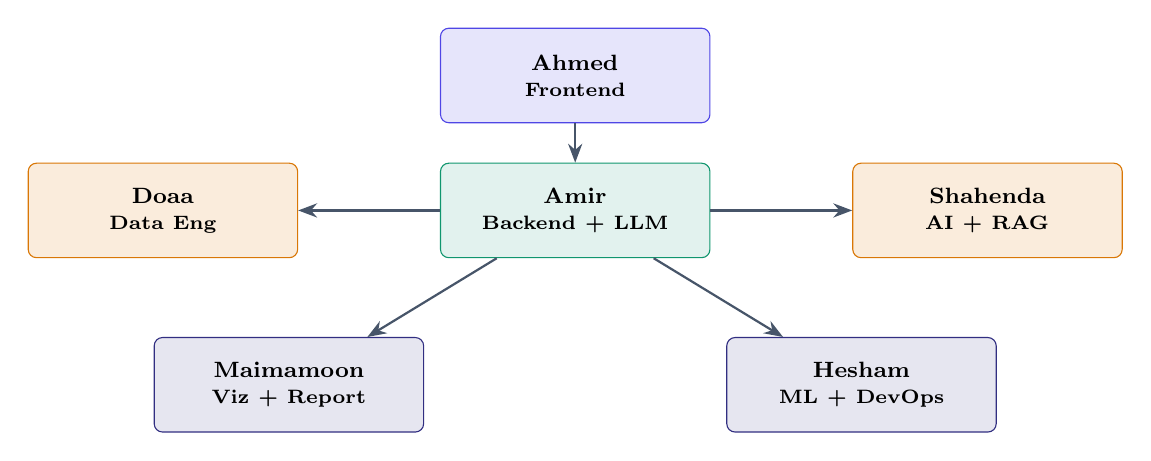
\begin{tikzpicture}[node distance=5mm and 8mm,
  o/.style={rounded corners=3pt,align=center,font=\footnotesize\bfseries,inner sep=6pt,minimum height=12mm,text width=3.0cm},
  a/.style={-{Stealth[length=2.4mm]},uaSlate,thick}]
  \node[o,fill=uaIndigo!14,draw=uaIndigo] (fe) {Ahmed\\\scriptsize Frontend};
  \node[o,fill=uaGreen!12,draw=uaGreen,below=of fe] (be) {Amir\\\scriptsize Backend + LLM};
  \node[o,fill=uaAmber!14,draw=uaAmber,left=18mm of be] (data) {Doaa\\\scriptsize Data Eng};
  \node[o,fill=uaAmber!14,draw=uaAmber,right=18mm of be] (rag) {Shahenda\\\scriptsize AI + RAG};
  \node[o,fill=uaIndigoD!12,draw=uaIndigoD,below left=10mm and 2mm of be] (viz) {Maimamoon\\\scriptsize Viz + Report};
  \node[o,fill=uaIndigoD!12,draw=uaIndigoD,below right=10mm and 2mm of be] (ml) {Hesham\\\scriptsize ML + DevOps};
  \draw[a] (fe) -- (be);
  \draw[a] (be) -- (data);
  \draw[a] (be) -- (rag);
  \draw[a] (be) -- (viz);
  \draw[a] (be) -- (ml);
\end{tikzpicture}
\caption{The ownership map. The backend core sits at the hub; data, AI,
visualization, and ML radiate out; the front end sits above.}
\label{fig:ownership}
\end{figure}

\section{Contract files}
Two files define the seams between people and are changed only by agreement,
because a change to either ripples across the split:

\begin{description}[style=nextline,leftmargin=0pt]
  \item[\textcolor{uaIndigoD}{\code{app/models/schemas.py}} (Amir)]
    The Pydantic request/response shapes. Every skill and route that crosses the
    API boundary speaks these types.
  \item[\textcolor{uaIndigoD}{\code{frontend/src/lib/api.js}} (Ahmed)]
    The client that calls those endpoints. It is the front-end mirror of the
    backend's schema contract.
\end{description}

\section{Collaboration model}
The split was designed for \emph{parallel, low-conflict} development: because
each member's files rarely overlap another's, commits can proceed independently
and merge cleanly. The shared contract files act as the coordination points ---
when the API shape changes, the two owners align, and everyone else consumes a
stable interface. This mirrors, at the level of team process, the same principle
that governs the software: clear boundaries, explicit contracts, and honest
communication across them.

\begin{uanote}[One system, six coherent slices]
The partition is not arbitrary. It follows the data as it flows through the
system --- ingest, retrieve, reason, visualize, predict, report, present --- so
each member owns a stage of a pipeline rather than a random scattering of files.
\end{uanote}

%=============================================================================
%  18_future.tex  -  Chapter 17: Future Work
%=============================================================================
\chapter{Future Work}
\label{ch:future}

Universal Analyst is a complete, working system, but its single-analyst,
single-session design leaves clear and deliberate room to grow. The roadmap
below follows naturally from the limitations stated in
Chapter~\ref{ch:security}, ordered roughly by impact.

\section{Persistence and accounts}
Sessions currently live in process memory. A persistent store --- a database for
session metadata and chat history, and durable storage for uploaded data and
generated reports --- would let analysts return to prior work, and would be the
foundation for user accounts and authentication.

\section{Multi-table and relational analysis}
Today a PDF or SQLite upload is reduced to its largest table. A natural extension
is first-class support for multiple related tables: retaining every table,
letting the analyst (or the model) express joins, and grounding answers across a
small relational schema rather than a single flat frame.

\section{Scaling the retrieval layer}
The bounded row-sampling strategy trades completeness for responsiveness at
upload time. Moving embedding to a background task with progress reporting would
allow exhaustive indexing of large datasets without blocking the request, and
approximate-nearest-neighbour tuning could keep retrieval fast at scale.

\section{Multi-tenancy and security hardening}
Authentication, authorization, per-user data isolation, and rate limiting would
turn the single-tenant tool into a shared service. Given the local-first
architecture, this can be added at the API boundary without disturbing the
grounding and validation core.

\section{Richer analytical skills}
The skill system is designed for extension. Candidate additions include
time-series forecasting, anomaly detection, automated feature engineering, and a
statistical-testing skill --- each following the established pattern of the model
proposing within a schema and deterministic code executing and measuring.

\section{Model flexibility}
The two-model strategy is configuration-driven, so supporting additional local
models --- or letting the operator choose per-task models --- is largely a matter
of configuration and light adaptation. A model-capability probe could tune
behaviour (for example, structured-output support) to whatever model is
installed.

\begin{table}[h]
\centering
\caption{Roadmap summary.}
\small
\begin{tabularx}{\linewidth}{@{}L{4.6cm} L{2.4cm} X@{}}
\toprule
\textbf{Initiative} & \textbf{Horizon} & \textbf{Primary benefit} \\
\midrule
Persistence \& accounts & Near & Return to prior work; foundation for users. \\
Multi-table analysis & Near & Real relational grounding. \\
Background indexing & Medium & Exhaustive retrieval at scale. \\
Multi-tenancy \& auth & Medium & Shared, secure deployment. \\
New analytical skills & Ongoing & Broader analytical coverage. \\
Model flexibility & Ongoing & Portability across local models. \\
\bottomrule
\end{tabularx}
\end{table}

\begin{uanote}[Growth without compromising the core]
Every item above can be added \emph{around} the grounding-and-validation core
rather than through it. The architectural decision to mediate everything behind
one backend is what keeps the roadmap additive instead of disruptive.
\end{uanote}

%=============================================================================
%  19_conclusion.tex  -  Chapter 18: Conclusion
%=============================================================================
\chapter{Conclusion}
\label{ch:conclusion}

Universal Analyst set out to answer a pointed question: can a language model make
data analysis faster \emph{without} making it less trustworthy? The system's
answer is a design, not a slogan --- a set of concrete engineering decisions
that together let the model be genuinely useful while never being the sole
authority on what the data says.

\section{What was built}
The project delivers a complete, local-first analytical workspace. A single
ingestion engine accepts five file formats; a deterministic profiler describes
the data exactly; a retrieval layer grounds every answer in the user's own file;
a streaming local model reasons over that grounded context; a validation-first
visualization engine renders only correct charts; a hybrid prediction pipeline
blends model reasoning with scikit-learn rigor; and a reporting engine exports
the whole session as a branded PDF. A thin, accessible React front end presents
all of this with exact readouts and honest error states.

\section{The through-line}
One idea runs through every chapter: \emph{the model proposes within a contract;
deterministic code disposes.} The model selects a chart type, a prediction
target, an algorithm, or a narrative --- but always inside a schema or a fixed
menu, and always subject to validation against the real data. Where the model or
the runtime fails, the system says so. This is what makes the tool an instrument
rather than a toy: every readout is exact and earned.

\begin{table}[h]
\centering
\caption{Objectives revisited.}
\small
\begin{tabularx}{\linewidth}{@{}L{5.0cm} C{2.2cm} X@{}}
\toprule
\textbf{Objective} & \textbf{Status} & \textbf{Evidence} \\
\midrule
Grounded question answering & \textcolor{uaGreen}{\textbf{Met}} & Per-session RAG
over profile, column, and row chunks. \\
Local, private inference & \textcolor{uaGreen}{\textbf{Met}} & Gemma\,4 via
Ollama; no data leaves the runtime. \\
Trustworthy visualization & \textcolor{uaGreen}{\textbf{Met}} & Schema-constrained
plans validated by \code{ChartFactory}. \\
Multi-format ingestion & \textcolor{uaGreen}{\textbf{Met}} & CSV, JSON, Parquet,
PDF, SQLite. \\
Actionable outputs & \textcolor{uaGreen}{\textbf{Met}} & Cleaning, prediction, and
PDF report skills. \\
Operational honesty & \textcolor{uaGreen}{\textbf{Met}} & The no-fabrication rule,
enforced end to end. \\
\bottomrule
\end{tabularx}
\end{table}

\section{Reflections}
Building the system as six coherent, contract-bounded slices proved as important
as any single feature: it let a team of six develop in parallel with minimal
conflict, and it mirrored in process the same clarity the software demands of
itself. The decision to mediate every capability behind one backend --- so that
grounding, validation, token accounting, and error honesty live in exactly one
place --- is what keeps the guarantees consistent and the roadmap additive.

\section{Closing}
Universal Analyst demonstrates that a local large language model, wrapped in the
right guardrails, can turn a raw dataset into an interrogable, trustworthy
workspace. It profiles honestly, retrieves faithfully, visualizes only what is
valid, predicts within bounds, and reports exactly what happened. It is, in the
end, what it set out to be: an instrument --- measured, grounded, and sharp.

\begin{center}
\vspace{6pt}
\begin{tikzpicture}
  \draw[uaLine,line width=0.8pt] (-3.2,0) -- (-0.6,0);
  \node[font=\itshape,text=uaSlate] at (0,0) {fin};
  \draw[uaLine,line width=0.8pt] (0.6,0) -- (3.2,0);
\end{tikzpicture}
\end{center}


% ============================ appendices ============================
\appendix
%=============================================================================
%  A_appendices.tex  -  Appendices
%=============================================================================
\chapter{Appendices}
\label{ch:appendix}

\section{Environment configuration template}
\label{app:env}
The complete configuration template shipped as \code{.env.example}. Copy it to
\code{.env} and adjust for the target runtime.

\begin{lstlisting}[style=bash,caption={\code{.env.example} (annotated).}]
# --- Server ---
HOST=0.0.0.0
PORT=8000
ENVIRONMENT=development           # development | production

# --- Ollama (LLM runtime) ---
OLLAMA_HOST=http://localhost:11434
# Docker (Ollama on host, backend in container):
# OLLAMA_HOST=http://host.docker.internal:11434

# --- Models ---
MODEL_NAME=gemma4:12b             # primary answering model (text + image)
ROUTER_MODEL_NAME=gemma4:e4b      # fast routing / classification
EMBEDDING_MODEL=all-MiniLM-L6-v2  # RAG embeddings

# --- RAG ---
MAX_CONTEXT_TOKENS=6000           # assembled RAG context budget

# --- Vector store (ChromaDB) ---
CHROMA_PERSIST_DIRECTORY=./chroma_data

# --- CORS ---
ALLOWED_ORIGINS=http://localhost:5173,http://localhost

# --- Multimodal chat ---
IMAGE_CHAT_ENABLED=true
MAX_CHAT_IMAGES=3
MAX_CHAT_IMAGE_MB=5
CONTEXT_WINDOW_TOKENS=256000      # front-end token-meter window
\end{lstlisting}

\section{The chat event protocol}
\label{app:events}
The \code{/chat} endpoint streams Server-Sent Events. Each event has a name and a
JSON \code{data} payload. The front end's \code{useChat} hook switches on the
event name to update the interface incrementally.

\begin{longtable}{@{}L{2.3cm} L{4.6cm} L{7.4cm}@{}}
\caption{Chat SSE events, payloads, and UI effect.}\label{tab:sseevents}\\
\toprule
\textbf{Event} & \textbf{Payload (illustrative)} & \textbf{UI effect} \\
\midrule
\endfirsthead
\multicolumn{3}{c}{\small\itshape (continued from previous page)}\\
\toprule
\textbf{Event} & \textbf{Payload} & \textbf{UI effect} \\
\midrule
\endhead
\midrule
\multicolumn{3}{r}{\small\itshape (continued on next page)}\\
\endfoot
\bottomrule
\endlastfoot
\code{skill} & \code{\{skill, reason\}} & Shows the selected skill. \\
\code{thinking} & \code{\{text\}} & Renders a reasoning affordance. \\
\code{action} & \code{\{action, detail\}} & Indicates a backend action. \\
\code{token} & \code{\{token\}} & Appends to the live answer. \\
\code{chart} & \code{\{spec / figure\}} & Adds a validated dashboard tile. \\
\code{usage} & \code{\{prompt, completion, total\}} & Updates the token meter. \\
\code{command} & \code{\{command, args\}} & Switches view / triggers download. \\
\code{error} & \code{\{message\}} & Displays the real error verbatim. \\
\code{done} & \code{\{\}} & Marks the turn complete. \\
\end{longtable}

\section{The chart-type catalogue}
\label{app:charts}
The twenty-six members of the \code{ChartType} enumeration, the single source of
truth for both the plan schema and the factory's validation.

\begin{lstlisting}[style=py,caption={\code{ChartType} enumeration.}]
BAR, LINE, SCATTER, PIE, HISTOGRAM, HEATMAP, BOX, VIOLIN, STRIP,
FUNNEL, FUNNEL_AREA, TREEMAP, SUNBURST, ICICLE, WATERFALL, AREA,
RADAR, DENSITY_HEATMAP, DENSITY_CONTOUR, SCATTER_GEO, CHOROPLETH,
SCATTER_MATRIX, PARALLEL_COORDINATES, PARALLEL_CATEGORIES,
SCATTER_3D, GAUGE, TIMELINE
\end{lstlisting}

\section{Repository structure}
\label{app:repo}
\begin{lstlisting}[style=bash,caption={Project layout (abridged).}]
DEPI_Graduation_Project_LLM_Driven/
  backend/
    app/
      api/            # chat, upload, sessions, clean, predict,
                      # visualizations, skills, health
      core/           # ingestion, chunker, profiler, session_manager
      eda/            # auto_eda
      llm/            # ollama_client, prompt_templates, token_counter
      rag/            # store, embedder, retriever, context_builder
      skills/         # cleaning, prediction, report, report_narrative
      skills_registry/# markdown skill definitions
      visualization/  # chart_factory, chart_types, export
      models/         # schemas, enums
      config.py, main.py
    tests/            # test_ingestion, test_profiler, test_visualization
    Dockerfile, requirements.txt, pyproject.toml
  frontend/
    src/
      components/     # chat, dashboard, upload, charts, sidebar, palette
      hooks/          # useChat, useSessions, useFileUpload
      lib/            # api, chartExport, reportDownload, tokenUsage
    Dockerfile, vite.config.js, tailwind.config.js, nginx.conf
  scripts/            # setup_ollama.sh, serve_frontend.sh
  docs/               # api_reference.md, deployment.md, latex/
  data/samples/       # example datasets
  main.ipynb          # cloud setup notebook
  docker-compose.yml, docker-compose.prod.yml, Makefile
  .env.example
\end{lstlisting}

\section{Technology summary}
\label{app:tech}
\begin{table}[h]
\centering
\caption{Complete technology stack.}
\small
\begin{tabularx}{\linewidth}{@{}L{3.2cm} X@{}}
\toprule
\textbf{Layer} & \textbf{Technology} \\
\midrule
Primary LLM & Gemma\,4 12B via Ollama (multimodal). \\
Router model & Gemma\,4 \code{e4b}. \\
Embeddings & \code{sentence-transformers} (\code{all-MiniLM-L6-v2}). \\
Vector store & ChromaDB (persistent, per-session collections). \\
Backend & FastAPI, Python\,3.12, \code{pydantic-settings}, \code{uvicorn},
\code{httpx}. \\
Data & pandas, numpy, pdfplumber. \\
ML & scikit-learn. \\
Visualization & Plotly, Kaleido. \\
Reports & ReportLab. \\
Frontend & React\,18, Vite, TailwindCSS, react-plotly.js, react-markdown,
lucide-react. \\
Infra & Docker Compose (dev + prod/nginx), Makefile, GitHub Actions, Ruff,
pytest. \\
\bottomrule
\end{tabularx}
\end{table}

\section{Glossary}
\label{app:glossary}
\begin{description}[style=nextline,leftmargin=0pt,itemsep=3pt]
  \item[\textcolor{uaIndigoD}{RAG}] Retrieval-Augmented Generation --- grounding a
    model's answer in facts retrieved from an external index rather than its
    weights.
  \item[\textcolor{uaIndigoD}{Semantic type}] The profiler's inferred role of a
    column (boolean, datetime, id, continuous, categorical, text), beyond its raw
    dtype.
  \item[\textcolor{uaIndigoD}{Chart plan}] A schema-constrained JSON description
    of a chart emitted by the model and validated before rendering.
  \item[\textcolor{uaIndigoD}{Skill}] A routed capability (analysis,
    visualization, cleaning, prediction, report, Q\&A) with Markdown guidance and
    a Python implementation.
  \item[\textcolor{uaIndigoD}{No-fabrication rule}] The commitment that the system
    shows real model output or a real error, never a placeholder.
  \item[\textcolor{uaIndigoD}{Structured output}] Ollama's mode for forcing
    JSON- or schema-valid model responses.
  \item[\textcolor{uaIndigoD}{Session}] One dataset-scoped analytical context,
    holding the DataFrame, profile, chat history, and generated charts.
\end{description}

\vfill
\begin{center}

\begin{tikzpicture}
  \node[font=\itshape\small,text=uaSlate]
    {Universal Analyst \;\textcolor{uaAmber}{\textbullet}\; Technical Documentation \;\textcolor{uaAmber}{\textbullet}\; DEPI Graduation Project};
\end{tikzpicture}
\end{center}


\end{document}
